%!TEX root = ../thesis_a4.tex
\chapter{Generative Symbolic Music}
\label{chap:symbolic}

\section{Introduction}

As long as computers have been available, a curiosity has prevailed as to whether computers are capable of being creative \citep{Cardoso2009}. Indeed the multidisciplinary area known as computational creativity \citep{Boden1998, Wiggins2006, Boden2009a, Boden2009, Colton2012} gathers researchers from artificial intelligence, cognition, philosophy and the arts, in order to investigate this lofty aspiration. In the wider sphere of computer music, algorithmic composition \citep{Jacob1996, Fernandez2013} endeavours to construct programs\footnote{Although most texts introducing algorithmic composition will be at pains to emphasise that algorithmic composition - in the context of some systematic application of rules for composing, like in Mozart's Dice game or in twelve-tone technique and serialism - in fact predates the computer.} that could automatically generate (or help generate) works of music for human listeners. With some composers, the goal is to model style conforming compositions \citep{Cope1987, Cope1991} so convincingly that they pass some interpretation of the Turing test \citep{Ariza2009}, while, others accept algorithmic composition for what it is - a different type of music, hence accepting all its limitations or possibilities, or as Pease puts it:

\begin{figure}
	\begin{center}
		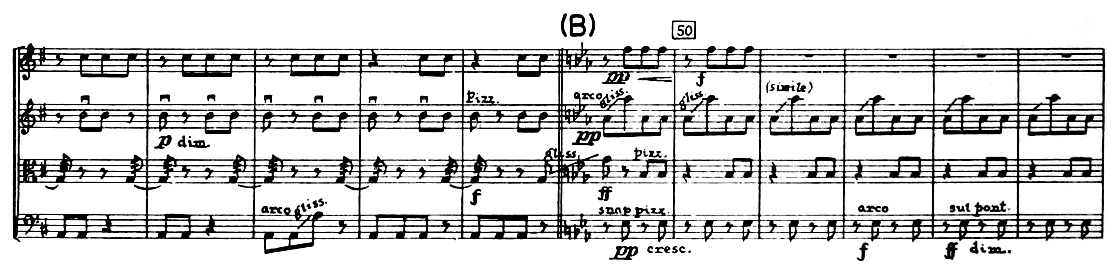
\includegraphics[width=\figSizeHundred]{ch03_symbolic/figures/illiac.jpg}
	\end{center}
	\caption[Excerpt from the \textit{Illiac Suite} (Lejaren Hiller)]{Excerpt from the Illiac Suite by Lejaren Hiller. Image from \cite{Morgan2015}}
	\label{fig:illiac}
\end{figure}

\blockcquote[]{Pease2011}{``\textit{Turing Test is largely inappropriate for the purposes of evaluation in Computational Creativity, since it attempts to homogenise creativity into a single (human) style}''}

In the early days of computer music composition, digital synthesis was only in its theoretical infancy, so algorithmic composition experiments typically involved generating some form of symbolic medium for later realisation as something audible. For instance, composers such as Hiller used supercomputers to generate a numerical computer score (\figref{fig:illiac}) which was then transcribed manually to staff notation and performed by a live string quartet \citep{Hiller1979}. Iannis Xenakis, in his treatise \textit{Formalized Music} \citep{Bradshaw1973}, explains how he harnessed supercomputer capability to generate large stochastic distributions that generated parameters for written compositions also to be realised by live performers. It is interesting to hear  how Xenakis calls attention to the role that computer programs play in \textit{assisting} him in his creative practice, rather than holistic generation of entire works\footnote{There are obvious parallels to be drawn here with Autechre's statement regarding their live work in \chapref{chap:dancemusic}.}:

\blockcquote[]{Cope2000}{``\textit{the computer has not actually produced the resultant sound; it has only aided the composer by virtue of its high-speed computations''}}

Later, with the advent of General \acrshort{midi}, music-oriented programming environments such as Max, \acrshort{pd} and OpenMusic were used to procedurally control note information and parameters of external hardware synthesisers and samplers automatically. One of my prior works \citep{Nuanain2014} explored tangible table-top interfaces modelled on the Reactable \citep{Jorda2005} for interactive control of real-time compositional algorithms, in a bid to expand the controller space offered by other real-time composition practitioners such as Karlheinz Essl \citep{Essl2014}. These experiments comprised a collection of Max/MSP patches that sent streams of algorithmically generated \acrshort{midi} control information to a virtual bank of synthesisers and samplers hosted in a \acrshort{daw}.

\section{Algorithmic Composition Techniques}

Programmatic techniques employed in algorithmic composition range from the very rudimentary (simple random number generators) to very sophisticated arrangements of agents borrowing from artificial intelligence. Algorithmic composition systems can be qualified as stochastic (the output is unpredictable), deterministic (the output is predictable) or hybrid, where one or more aspects of the system are determined.

There exists a wealth of conceptual approaches exist for algorithmic composition that have fallen in and out of flavour over the years. We summarise key ones here that we feel are representative of the current state of the art and pertinent to the arguments put forth within the thesis. For a thorough treatment of historical methods for algorithmic composition we suggest consulting the Computer Music Tutorial \citep{Roads1996} or surveys reported by \cite{Fernandez2013} and \cite{Papadopoulos1999}.

\subsection{Stochastic Processes}

Stochastic processes are largely concerned with strategic applications of probabilistic procedures. When composers defer some aspect of their creative activity to some element of chance they are invoking a stochastic process; whether this be the flip of a coin to choose which section to enter in a large musical structure or using a random number generator to select pitch values on their synthesiser, for example.

\subsubsection{Probability Distributions}

Composers using random processes in a serious way (like Hiller and Xenakis) naturally gravitate towards methods of influencing the outcomes in some systematic manner. They  utilise probability table lookups to shape a specified probability distribution geared towards a desired musical elemental goal. Most computer music oriented software environments have some sort of facility for creating such distributions interactively, and in fact Max/MSP provides a visual table object for drawing distributions explicitly. They can be used to create standard mathematical distributions such as linear, bell-shaped, skewed etc., and \textit{The Computer Music Tutorial} \citep{Roads1996} gives derivations for many of them in the chapter dealing with algorithm composition. \cite{Ames1990a} also gives insight into similar statistically grounded modes of composition.

Sometimes a more musically specific distribution is required. Using the example of a probability distribution influencing the outcome of pitches available from the 88 notes of a conventional keyboard, we could envisage a distribution that only allows notes from the major scale, and favours the root, fourth and fifth as prevalent in many Western musical idioms.

Thinking further about this, if an analysis can be performed on a suitable set of representational data (such as a score, \acrshort{midi} file or features extracted from audio), the distribution of pitches in the scores of Chopin or based on pitch histograms in a selection of Javanese Gamelan recordings, one may surmise a very elemental manner of encapsulating the notion of style within a composition system. 

Instinctively however, the fundamental feature lacking is any information about the appropriateness of the pitches given the surrounding context and overall trajectory. One extremely applicable method of addressing this is through the use of Markov processes.

\subsubsection{Markov Processes}
\label{sec:markov_chains}

A Markov chain is a probabilistic system that satisfies the Markov property of memorylessness. It consists of a set of discrete states with each state having an associated probability weighting of moving to every other state in the system. At any point in discrete time, the probability of a future event is solely determined by the current state (or a few states depending on the \textit{order}) of the system without knowledge of the preceding past events. This can be expressed more formally by \eqnref{eq:markov}.

\begin{equation}
  \label{eq:markov}
  \begin{gathered}
P=(X_{t+1}|X_{t}=x_{t},X_{t-1}=x_{t-1},...,X_{0}=x_{0}) \\
=(X_{t+1}|X_{t}=x_{t})
  \end{gathered}
\end{equation}

where $X_t$ is the state occupied by the state machine at time $t$ in its discrete history. To build a Markov chain, a transition matrix is defined that determines the probability of moving from one state to each other, often by analysing or modelling some real world examples. The order (i.e. the number of states in the right hand side of the second line of \eqnref{eq:markov}) of this transition matrix is the number of states that are considered when determining the probability of the next state. A first order Markov chain, for example, considers the probability of jumping to the next state based on the current state, while a second order chain would use the current state and the previous state in determining where to move to next.

Markov chains have enjoyed widespread application in simulating stochastic processes, and in music they are employed routinely for algorithmic composition \citep{Fernandez2013, Eigenfeldt2009, Jorda2016}. A simple Markov chain for generating notes in a particular style could be achieved by building a transition matrix from the number of times the root note of a scale transitions to every other note in a corpus of \acrshort{midi} files. This could be expanded to include a concurrent transition matrix that contains probability of transition of observed note rhythm values. Some of our colleagues in GiantSteps have also addressed drum pattern generation with a system of Markov Chains derived from style specific corpora addressing various strands of electronic dance music \cite{Jorda2016, Gomez-Marin2016}.

With The Continuator, \cite{Pachet2002} has garnered considerable exposure in the application of Markov chains in call and response style interaction with a human performer\footnote{And we shall see later \cite{Biles1994} achieves something similar with his means of ``trading fours'' with a real-time listening \acrshort{ga}.}. The allure of Pachet's work has been its satisfaction of a number of Turing style tests \citep{Pachet2008}. More recently its successor \acrshort{ai}, FlowMachines \citep{Pachet2008a}, has stirred up great publicity\footnote{\url{http://www.flow-machines.com/tag/flow-machines-press/}} with its generation of the first artificially intelligent pop song\footnote{With the caveat being a human wrote the lyrics and arranged and performed the final work.}. In their usage of Markov chains, they have acknowledged their facility for modelling temporal phenomena such as music, but emphasise the challenge in reconciling them for interactive control. To solve this they have proposed a class of hybrid Markov chain system that includes elements of constraint satisfaction, known as an \acrfull{emc} \citep{Pachet2011}, proving fundamental for chord generation in the Continuator \citep{pachet2001finite, barbieri2012markov}.

Music generated by Markov Chains can be deceptive in their `low-level' convincingness but it is still very localised in contrast to larger human-composed works with careful macroscopic attention to form. As \cite{Collins2011a} comment on The Continuator: ``it is fundamentally parasitic on the duration data passed to it'' and has ``difficulty with longer-term structure''.

To combat this the composer can increase the order of the Markov system - thereby lengthening the `memory' of consideration in the state machine - or similarly lengthening the size of the snippets of symbolic music atoms that are to be used for chaining, but the results still baulk at a point. As Roads observes when studying hymns generated with a Markov chain by \cite{Brooks1993}. 

\blockcquote[]{Roads1996}{``\textit{...low-order chains generated meandering, random melodies, while high-order chains consist of parts of the original hymns spliced together, such as the first half of one hymn crudely spliced onto the second half of another hymn. This can be explained as a strong probabilistic tendency towards coherence over several notes that is broken suddenly by a more unlikely event, at which point a new coherent melody starts''}}

Jordà concurs in his own evaluation of his own compositions for live computer music generating jazz chord progressions. 

\blockcquote[]{Jorda1991}{``\textit{Markov music usually presents a very short correlation, sounding much better over brief fragments, than over long ones.}}

With these criticisms in mind, maybe this makes the case for hybrid systems that can scale with the demands of larger scale computer music composition. By invoking a layered approach with multiple agents perhaps taking the role of a meta-composer for the purposes of coherent musical form. In fact Eigenfeldt does talk about this in the context of musical meta-creation \citep{Eigenfeldt2016}, and prior to that defines some mechanism that is rudimentarily capable of doing something to that effect. In \textit{GESMI} - the Generative Electronica Statistical Modeling Instrument \citep{Eigenfeldt2013} - for example, expert annotations of aspects of electronic dance music including subdivisions into section labels such as `lead-in', `intro', `verse' and `breakdown' are used by a genetic algorithm to dictate higher-level surface features while Markov chains generate localised motifs as usual. In another work \citep{Eigenfeldt2016a}, another high-level meta-agent defines a series of parametric curves that affect overall compositional aspects such as speed, density and complexity that are adhered to by other reactive generative agents.

\subsection{Formal Grammars}

Continuing with the goal of epitomising style in computational models and generative procedures, we turn to another approach that tries to achieve this using language theory. Formal grammars have long been used to interpret hierarchical relationships in syntactical aspects of language \citep{Chomsky1957}, and are an essential element of compiler theory and programming language design \citep{garshol2003bnf, wirth1996compiler}.

The controversial debate continues as to whether music can really be considered a universal language \citep{Campbell1997, Savage2015} but, nevertheless, applying formal grammar theory has enjoyed considerable utility in the systematic analysis of musical concepts as well as generative tasks. In his famous Harvard lecture series ``The Unanswered Question''\footnote{\url{https://youtu.be/MB7ZOdp__gQ}}\citep{bernstein}, the conductor Leonard Bernstein pondered whether music could be characterised using Chomsky’s formal generative grammars \citep{Chomsky1957}. Subsequently inspired by this hypothesis, musicologist Fred Lerdahl and linguist Ray Jackendoff \citeyearpar{lerdahljackendoff} joined forces to compile ``A \acrfull{gttm}'', one of the most complete compendiums to classify Western classical music using grammar techniques. A dense and complex work, it nevertheless provides a methodological framework for understanding what we hear when we listen to common practice works. The metrical structure rule for instance, positions beats in a tree structure such that it accounts for the natural strong and weak grouping of accentuation that occurs at different metrical levels of pulse as can be seen in \figref{fig:gttm}.

\begin{figure}
	\begin{center}
		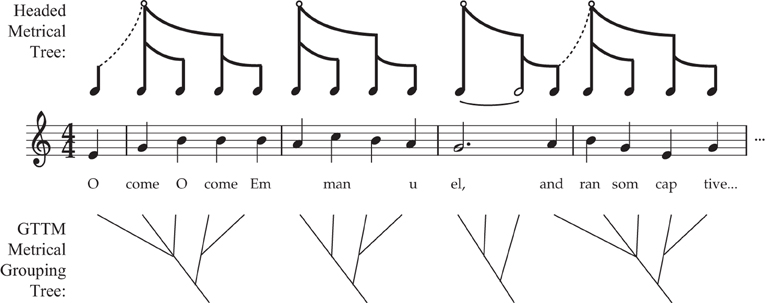
\includegraphics[width=\figSizeHundred]{ch03_symbolic/figures/metricalhierarchy.jpg}
	\end{center}
	\caption[Generative Theory of Tonal Music Metrical hierarchy grouping]{\acrshort{gttm} metrical hierarchy grouping. Image from \cite{Fitch2013}.}
	\label{fig:gttm}
\end{figure}

Lerdahl and Jackendoff’s \acrshort{gttm} represents, as Roads suggests, an “analysis of syntactic structures” where musical events are parsed into syntactic hierarchical structures \citep{Roads1996}. Conversely he contrasts the analytical viewpoint with the synthetic: “starting from a specification of large-scale syntactic structure fill in the details for each of these structures”.

The \acrshort{gttm} essentially comprises an analysis or distillation of style, the style loosely being common practice era Western art music. Composer David \cite{Cope1991} has, using his musicological expertise, performed a similar analysis of music from this era, but with a more finely grained focus, initially on Bach chorales. More importantly the primary goal of this analysis is to inform the eventual synthesis of style. Cope distills his \acrfull{emi} \citep{Cope1987} process into three critical stages that mirror Roads’ observations regarding duality of musical application involving formal grammars. In any case he identifies them as:

\begin{itemize}
	\item Deconstruction - segmentation and analysis of existing representative work
	\item Signatures - identifying demonstrative motifs and traits that distinguish a stylistic genre or composer’s proclivity
	\item Compatibility - recombine deconstructed elements into fresh cohesive and coherent musical works
\end{itemize}

Controversy aside, what Cope perhaps highlights most of all is the role of the designer in building computer composition systems. As is evident, building a software that can achieve the output of \acrfull{emi} is no easy feat, demanding a Bach scholar with knowledge of the nuances of voice leading, counterpoint, as well as computational musicological skills that include awareness of \acrshort{ai} methods and programming in \acrshort{lisp}\footnote{\acrfull{lisp} is a programming language with a long association in the field of \acrshort{ai} and by extension, computer music \citep{taube1991common, taube2004notes, assayag2006computer}.} for example. On a more philosophical note, it should follow that the designer then must impart some aesthetical footprint on works produced by such systems. So if we can hear which part reveals a piece to be Bach, then which part is the designer? Which part is the computer? 

Cope has available 5000 examples of computer generated Chorale in \acrshort{midi} format on his website, and has continued his experiments to include more larger scale works extending into the common practice era and beyond (e.g. Mozart and Mahler \citep{Muscutt2007, cope2009hidden}). His efforts have had an enduring and frequently contentious impact not only in academia \citep{Wiggins2008} but also in the public’s psyche; by addressing well known and easily identifiable stylistic goals (verifiable once again with musical style Turing tests)   he establishes clear markers in the sand for what is achievable with algorithmic composition. 

\subsection{Genetic Algorithms}


\acrfullpl{ga}, as introduced in seminal works by \cite{Holland1975} and \cite{Goldberg1989}, are a class of heuristic search solutions modelled on the theory of natural selection \citep{koza1992genetic, Srinivas1994}. Along with artificial neural networks and emergent systems they can be classified as a biologically inspired computing method that employs some well understood  process from natural sciences to help solve a more complex computational task \citep{Mitchell1998}.

In a \acrshort{ga}, potential solutions to a conceptual problem are encoded with a genome string representation (usually with binary bitstrings). Using a series of genetically-inspired operations such as crossover and mutation these strings are ``evolved'' until their quality reaches a satisfactory level, hence performing an implicit search sweep over a large space of candidates.  Central to the operation of evolutionary algorithms and determining genomic quality is the \textit{fitness function}, which determines the individuals that are allowed remain in successive populations. Naturally effective representations are important to ensure effective use of evolutionary algorithms - a badly defined encoding can skew the performance towards that of exhaustive search. 

Several logical stages are involved in a genetic algorithm which we now discuss in turn:

\paragraph{Initiation:}
To initiate the search space, a population of individuals is generated randomly, though some rules-based procedures can assist in “kick starting” a faster, more informed process.

\paragraph{Fitness:}
The fitness function is a problem-dependent evaluation procedure that determines the suitability of the candidate solution to the problem. There are no hard and fast rules as to what determines a “good” fitness function; this is - along with specifying an appropriate representation - part of the craft in evolutionary algorithms. An alternative is to use an interactive fitness function, which involves using an external agent (typically a human critic) to determine suitability of candidates. 

\paragraph{Selection:}

In accordance with Darwinist theory, the fittest $f$ individuals are more likely to be chosen for reproduction and generation of future population members. This is in essence probabilistic, and one popular selection schema is roulette wheel selection, or fitness proportionate selection. Here, the probability assigned to an individual is given by the proportion of the individual fitness to the overall population (\eqnref{eq:roulette}).

\begin{equation}
\label{eq:roulette}	
p_{i}=\frac{f_{i}}{\sum_{i=1}^{N}f_{i}}
\end{equation}

Where $p_i$ is the probability of individual $i$ being chosen and $f_i$ is the fitness of that individual.

Roulette wheel selection derives its nickname from being akin to reserving a portion of a spinning roulette wheel in a casino. In \figref{fig:roulette} this can be graphically compared to truncation selection which simply selects the top \textit{N} members from the list when sorted by fitness.

To create the offspring, genetic operators are applied to the parent individuals, the two most common being:
\begin{itemize}
	\item \textit{Crossover} - pick a splice point s in the bit strings of the genome, take bits 0 - s from parent A and combine with bits s - n from parent B.

	\item \textit{Mutation} - a certain (small) portion \ of the newly generated population is chosen at random and within these individuals a random bit is flipped. As in nature, the mutation procedure allows for genome sequence combinations that may not occur using crossover alone.
\end{itemize}

\begin{figure}
	\begin{center}
		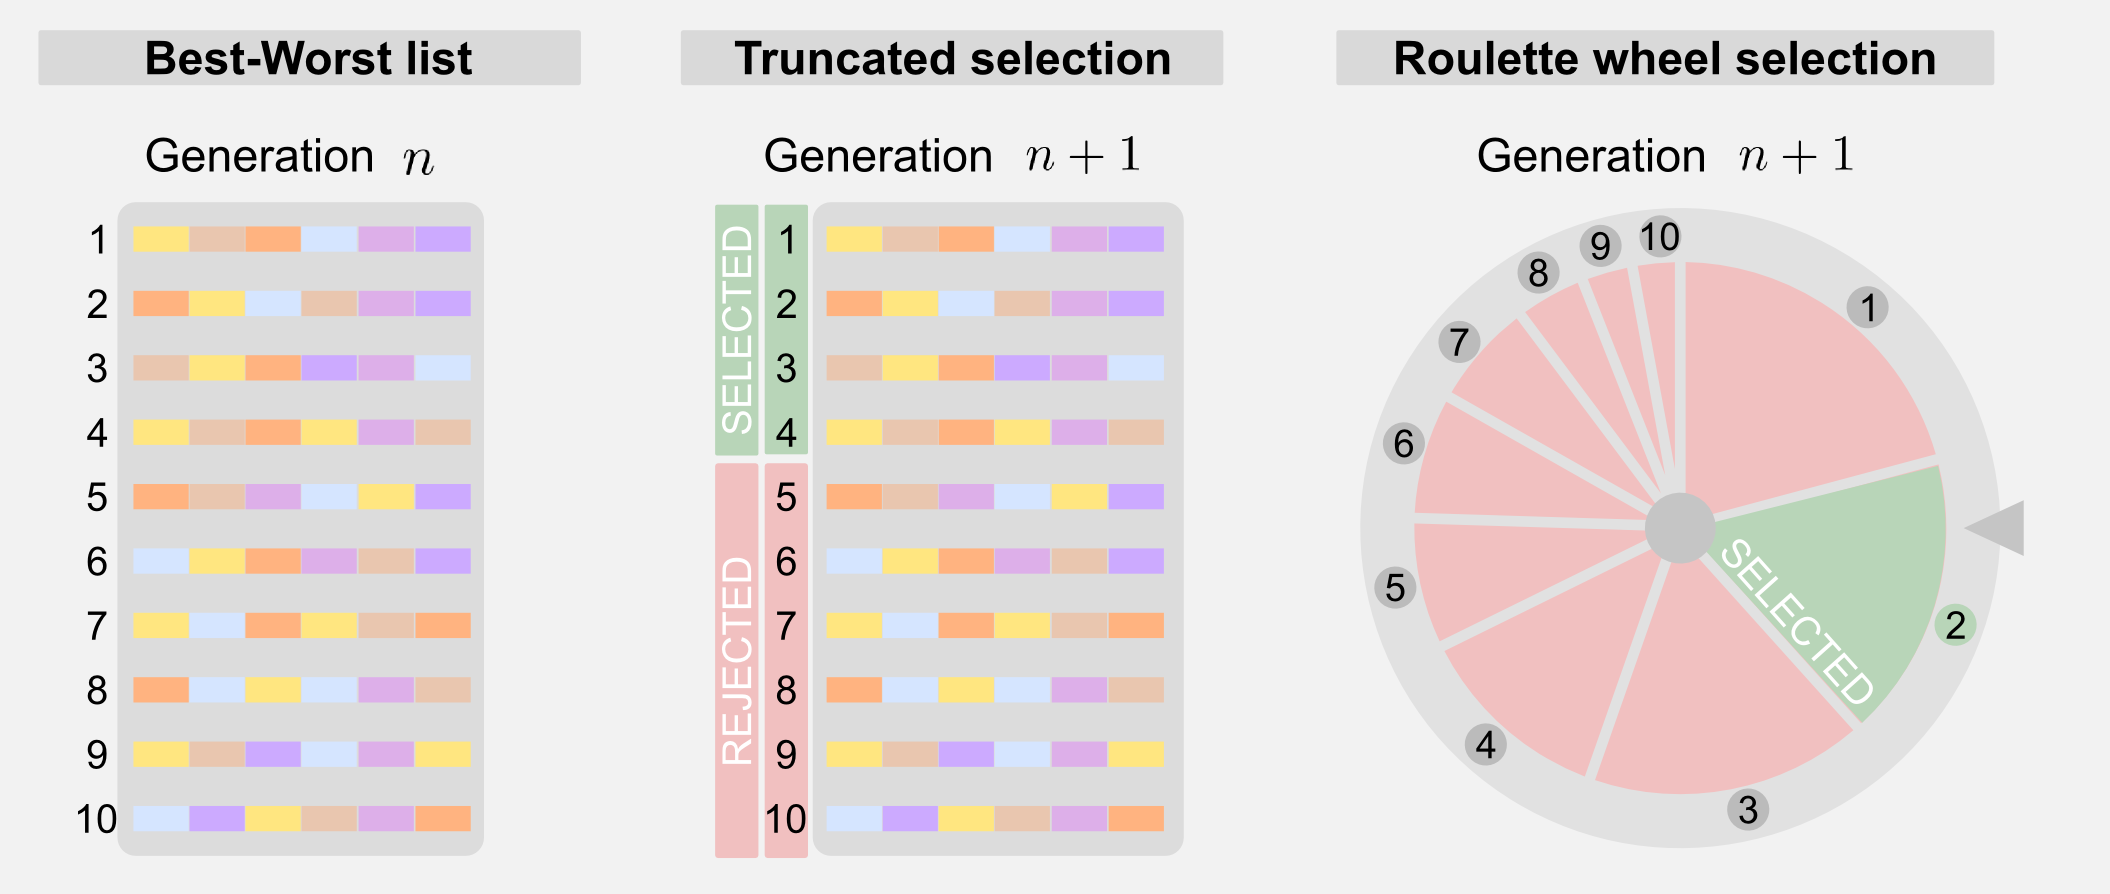
\includegraphics[width=0.9\textwidth]{ch03_symbolic/figures/selection.png}
	\end{center}
	\caption[Truncation and roulette wheel selection in a genetic algorithm]{Sorted best to worst list of candidates (left). Truncated selection of top 4 candidates (middle). Probabilistic roulette wheel selection (right). Image from Dissecting Reinforcement Learning\footnote{\url{https://mpatacchiola.github.io/blog/2017/03/14/dissecting-reinforcement-learning-5.html}} }
	\label{fig:roulette}
\end{figure}

\subsubsection{Evolutionary Music}

Genetic algorithms have certain qualities that make them an attractive choice for artificial creativity, so much so that there exists an ardent strand of research devoted entirely to what has come to be known as “evolutionary art” \citep{Romero2008, McCormack2013} and furthermore, evolutionary music \citep{Miranda2007a} .

Undoubtedly, they are an elegant and easy to comprehend search heuristic, and the underlying concept of generating a bunch of candidate solutions that hopefully converge on some ideal is appealing to the process of an artist. So too is the idea of the interactive fitness function, where humans can directly appraise potential candidates subjectively. Naturally this is the most optimal method aesthetically but the slowest method performance-wise, especially in highly temporal domains such as sound and vision, where it is typically referred to as the “fitness bottleneck” \citep{Todd1999, Biles2001, Gartland2003}. 

One of the most well known applications of genetic and evolutionary algorithms to music has been Al Bile’s GenJam system \citep{Biles1994,Biles2002,  Biles2003, Biles2007} which interactively generates streams of monophonic solo melodies in bebop jazz style.  It is a classic example of an interactive genetic algorithm \figref{fig:genjam}, where the composer considers himself a “mentor” to the system, actively incrementing and decrementing fitness of generated phrases as they arise in real time from the program. Internally, the genetic algorithm actually maintains two populations of structures. The phrase population contains a list of indices that reference measures in the measure population. A measure is considered a short eight-note phrase of \acrshort{midi} pitch values, with special symbols for silence and held notes.  One of GenJam's unique feature is the ability to “trade fours” with the live performer whereby pitch detection is performed on a monophonic input source, and the phrase that is altered using genetic modifiers is played back to the performer.

\begin{figure}
	\begin{center}
		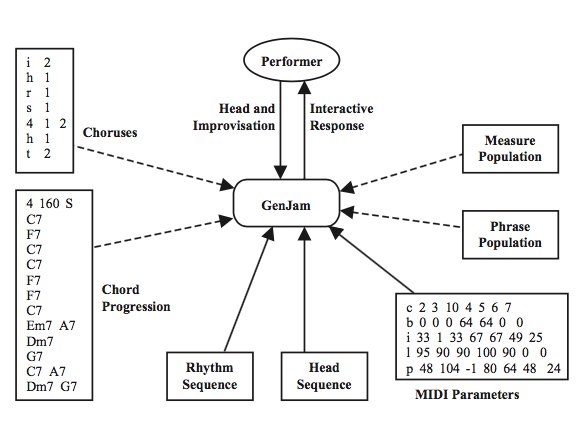
\includegraphics[width=0.8\textwidth]{ch03_symbolic/figures/genjam.png}
	\end{center}
	\caption[GenJam architecture]{GenJam architecture with different populations and interaction with performer. Image from \cite{Miranda2007a}.}
	\label{fig:genjam}
\end{figure}

Now that we have seen a glimpse of basic methods for symbolic algorithmic composition, we will begin our study of symbolic generation focussing on rhythm using computer processes. We will turn our attention to some key works presented in the literature and describe a new method of target-based rhythmic pattern generation using genetic algorithms. An evaluation will unearth the feasibility of such methods for rhythm pattern generation and the limitations that can be identified that informs a revision of the models used.\

\section{Symbolic Rhythm Generation}

\subsection{Representation}

As evident from such designs as Léon Theremin's `Rhythmicon', the Wurlitzer `Sideman' and Raymond Scott's `Rhythm Synthesizer'\footnote{The Rhythm Synthesizer would sow the seeds for a later drum machine called `Bandito the Bongo Artist' which would be used on the ground-breaking proto-ambient record \textit{Soothing Sounds for Baby}\citep{Collins2011a}} \citep{Tindale2009, Malmberg2010, Arar2013}, there have been many esoteric early incarnations at building and incorporating drum computers, with these strange experiments in the early half of the 20th century paving the way for a more unified design aesthetic emerging towards the latter half. 

\begin{figure}
	\begin{center}
		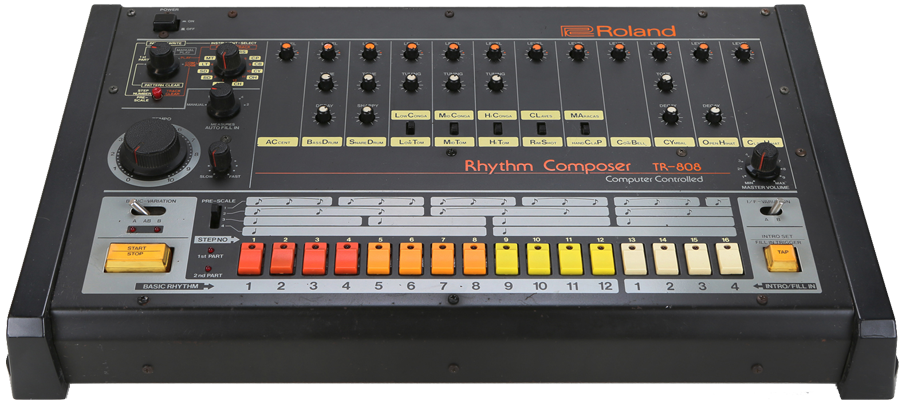
\includegraphics[width=0.75\textwidth]{ch03_symbolic/figures/tr-808.png}
	\end{center}
	\caption[Roland TR-808 drum machine]{Roland TR-808 drum machine.}
	\label{fig:tr-808}
\end{figure}


Most notably, one can not underestimate the profoundly influential impact of the designs of Ikutaro Kakehashi and the Roland Corporation on the shape and history of electronic music and its culture. Originally considered a commercial flop due to its perceived inauthentic synthesis of natural drum sounds, the Roland TR-808 drum machine (\figref{fig:tr-808}) has since become the icon of post 1980s dance oriented music, and its distinctive synthetic character soon became synonymous with techno and house styles \citep{theberge1997any}.

The TR-808 was intended as a rhythm accompaniment device, and as such was designed to be easy to use by non drummers. Its operation involved selecting the required drum sound and inputting a pattern using a row of 16 buttons corresponding to discrete points in time based on a global tempo. This binary based approach has continued on into computer music platforms and virtual instruments. 


This simple but concise metaphor of representing basic patterns has been adapted also in the literature dealing with the musicological study of rhythm, most notably by \cite{Toussaint2013} who has carried out considerable research into geometric approaches for rhythm analysis and similarity. The binary input mechanism is clearly a convenient medium for transferring to computational analysis while remaining descriptive and intuitive for human comprehension.  \figref{fig:reps} shows how a particular rhythm can be represented in a number of different symbolic representations including traditional staff notation forms.

\begin{figure}
	\begin{center}
		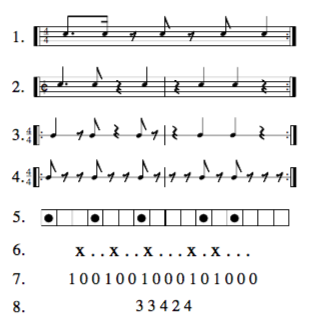
\includegraphics[width=0.55\textwidth]{ch03_symbolic/figures/reps.png}
	\end{center}
	\caption[Different forms of symbolic rhythm representations]{Different forms of symbolic rhythm representations. Image from \citep{Toussaint2003}.}
	\label{fig:reps}
\end{figure}

The fifth form in the figure, the most familiar to drum machine interfaces, is referred to as the \acrfull{tubs}. It is considered easier by many ethnomusicologists in depicting and grasping complex rhythmic structures such as polyrhythms not typical in Western Art Music \citep{nzewi2008musical, koetting1970analysis}.  

Continuing in this line, other representational schemes have been devised in attempt to represent rhythms in a more holistic and natural manner, given its cyclical and hierarchical centricity. Often rhythms are portrayed using a circle or necklace system with beats and onsets occupying geometric portions of the structure, as can be seen in \figref{fig:necklace}. These are frequently used to depict more complex rhythmic patterns that exist in African and Latin traditions, giving a different perspective and insight into their latent balance and symmetry.

\begin{figure}
	\begin{center}
		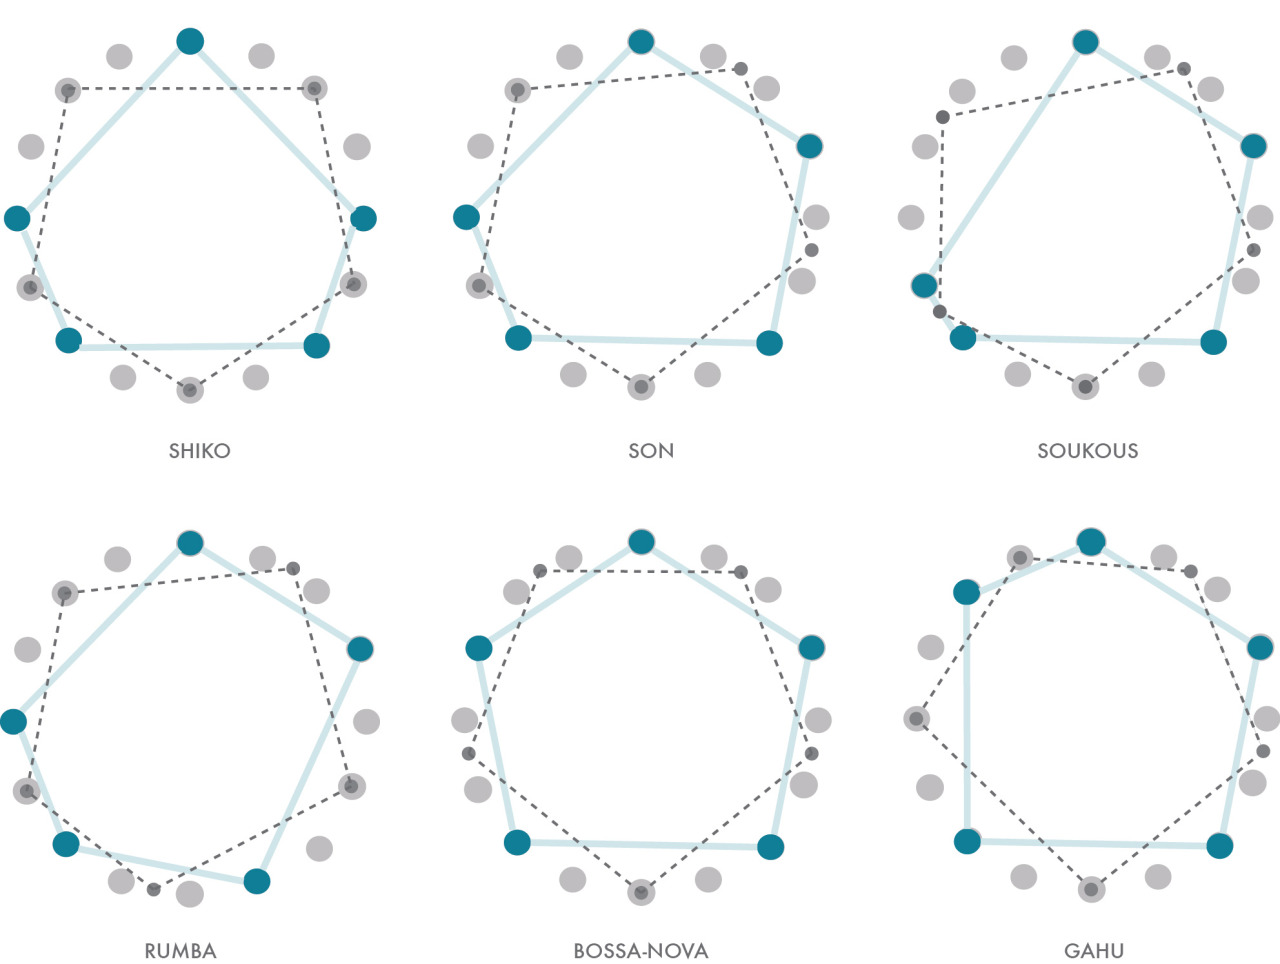
\includegraphics[width=\figSizeHundred]{ch03_symbolic/figures/necklace.jpg}
	\end{center}
	\caption[Necklace depictions of some popular rhythms.]{Necklace depictions of some popular rhythms. Image from Ethan Hein\footnote{\url{http://www.ethanhein.com/wp/2015/beats-and-scales/}}.}
	\label{fig:necklace}
\end{figure}

These circular representations have proved alluring for computer music practitioners, and a number of rhythm focussed applications have been developed exploiting this necklace paradigm. Xronomorph \citep{Milne2015a, Milne2016}, provides an environment for experimenting with rhythms that conform to mathematical properties of perfect balance and well-formedness. As a unified mobile application, Rhythm Necklace\footnote{\url{http://rhythmnecklace.com/}} is a visually appealing application for iPad for experimenting with geometrical approaches to rhythm generation.

\begin{figure}
\centering
\begin{subfigure}[b]{1.0\textwidth}
   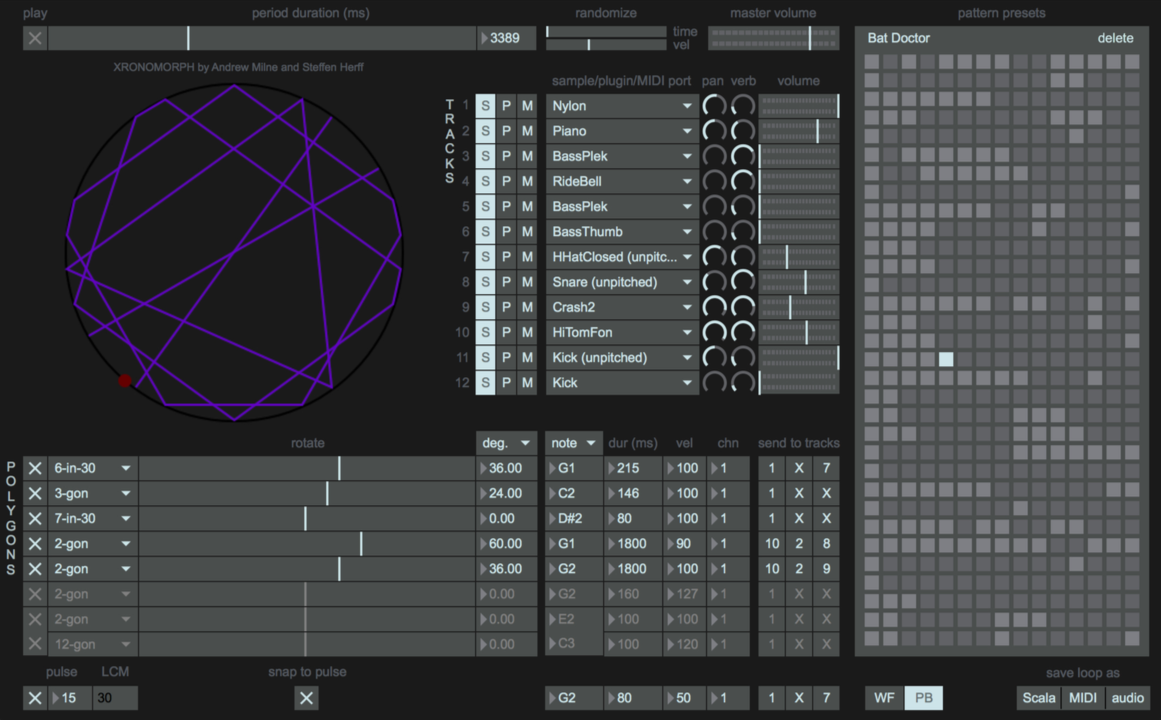
\includegraphics[width=1\linewidth]{ch03_symbolic/figures/xronomorph.png}
   \caption{}
   \label{fig:Ng1} 
\end{subfigure}

\begin{subfigure}[b]{1.0\textwidth}
   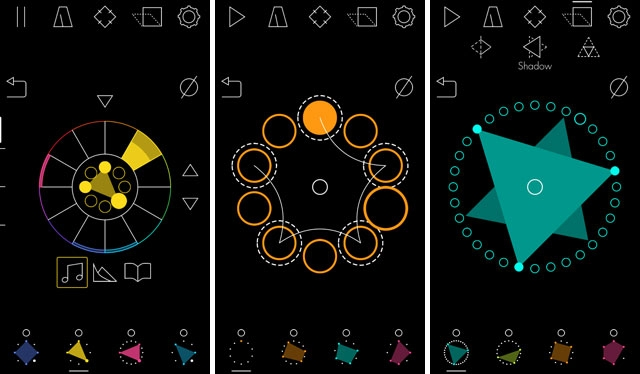
\includegraphics[width=1\linewidth]{ch03_symbolic/figures/necklace2.jpg}
   \caption{}
   \label{fig:Ng2}
\end{subfigure}

\caption[Necklace representation in Xronomorph and Necklace interfaces]{(a) XronoMorph interface. Image from \cite{Milne2016}., (b) Rhythm Necklace app. Image from Ethan Hein\footnote{\url{http://www.ethanhein.com/wp/2015/rhythm-necklace/}}.}
\end{figure}

\subsection{Measuring Rhythmic Similarity}

One of the primary tasks that has dominated symbolic rhythm study has been the formalisation of methods for measuring the degree of similarity between two rhythmic patterns. It was previously shown how natural rhythms can be distilled down to a very simple representational form suitable for computational analysis (and hopefully generative composition).

Obviously, there is a wealth of knowledge and systematic approaches for measuring similarity borrowing from information sciences when dealing with computer readable data, or in particular, strings. Methods of comparing strings, or string metrics, are an essential aspect of coding theory. Symbolic rhythmic study has adapted many of these metrics for its analysis and \cite{Toussaint2004} has summarised many of the key matching techniques. Superficially, we can take a distance measure, feed it some rhythms encoded as binary strings and do some basic normalisation/algebra to convert it to some degree of “similarity”.

The key question here is how do these objective information metrics compare with the cognitive human impression of similarity? With this very shallow abstraction of what a rhythm is, we must surely lose a great deal of latent information that undoubtedly must contribute to similarity perception; consider the influencing factors of accentuation, swing, timing imperfections, instrumentation, timbre, production, genre and surely, culture. 

Regardless, the foundations of understanding rhythmic similarity need to begin somewhere. We turn our attention now to methods of estimating similarity of simple binary string representations of rhythmic structures and discuss their relevance and application for generative purposes in a practical system in due course.

\subsubsection{String Similarity and their Application to Rhythms}

\label{sec:distance_measures}

\begin{figure}
	\begin{center}
		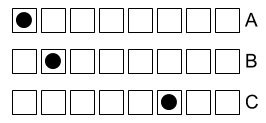
\includegraphics[width=0.45\textwidth]{ch03_symbolic/figures/hamming_comparison.png}
	\end{center}
	\caption[Hamming distance comparison for three different patterns ]{Same hamming distance for three different patterns}
	\label{fig:hamming_comparison}
\end{figure}

The primary advantage of the simple binary representation exemplified by the \acrshort{tubs} notation is its malleability for simple bit comparison and string analysis using common algorithms. We summarise a number of them here for clarification, but Toussaint  offers a more thorough synopsis of many of them and their application to rhythm.

\paragraph{Edit Distance:} The edit distance or Levenshtein distance is a widely-used measure of difference between two strings of information. It counts the number of insertions, deletions and substitutions required to transform one string into the other. The  Levenshtein distance between the two strings “kitten” and “sitting” for example returns 3, based on two substitutions and one addition. The edit distance can operate on strings of differing lengths, and is solved using recursion or dynamic programming techniques.

\paragraph{Hamming Distance:} The hamming distance counts the number of positions in which two equal length strings differ. A simple measure that is easy to compute for the machine and easily comprehensible for the human. Hence it is a restricted version of the edit distance, limiting itself solely to substitutions of symbols.

\paragraph{Swap Distance:} As \cite{Toussaint2013} notes, one of the problems with the edit distance and the Hamming distance is that they don’t capture the horizontal aspect of string similarity so well. In \figref{fig:hamming_comparison} for instance, comparing string A to string B and string C both return a distance of 2, even though comparing them horizontally they are clearly very different.

To this effect, Toussaint proposes the use of the swap distance, actually borrowed from similar computations that take place in the realm of bioinformatics, to capture the number of placewise shifts to make one string match the other. as he did in his study of African ternary rhythms \citep{Toussaint2003}. In the simple case of binary encoded rhythms with equal number of onsets or 1s - known as one-to-one mapping - the distance can be computed by summing the absolute differences in their indices \citep{Toussaint2016} - essentially the L1-Norm or ``Manhattan'' distance (\eqnref{eq:swap}) when considering element $a_i$ and $b_i$ from two strings $A$ and $B$.

\begin{equation}
\label{eq:swap}
	\mathcal{D}_\mathrm{S}(A,B) = {\sum_{i=1}^{N}|a_i-b_i|}	
\end{equation}

Of course natural rhythms can have different numbers of onsets and this does make computing swap like similarity considerably more complex. To handle this extended case of many-to-many, \cite{Diaz-Banez2004} have applied what is known as the directed-swap in their analysis of flamenco patterns, which stipulates, when comparing a pattern A with more onsets than pattern B that:

\begin{enumerate}
	\item Each onset in pattern A must move to an onset in pattern B.
	\item Every onset in pattern B must receive at least one onset from pattern A.
\end{enumerate}

In \figref{fig:swapvshamming}, we can see a visual comparison of the directed-swap distance as compared to the Hamming distance, as well as the different distance values they return. Conceptually, we can at least surmise that the directed-swap, with its ability to encode the horizontal displacement of onsets, should give a richer description of the similarity between two rhythms, such as embodying an impression of the syncopation introduced. if we were to move between both patterns.

\begin{figure}
	\begin{center}
		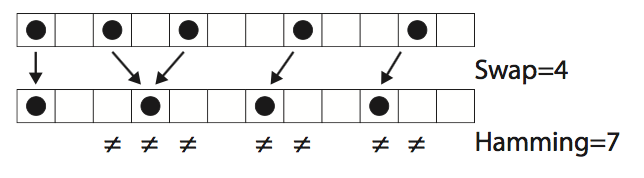
\includegraphics[width=0.65\textwidth]{ch03_symbolic/figures/swap_vs_hamming.png}
	\end{center}
	\caption[Swap and Hamming distance compared.]{Swap and Hamming distance compared.}
	\label{fig:swapvshamming}
\end{figure}

Actually computing this distance is also a more involved task. One proposed, which works in $O(n^{2})$ time, solution is to consider the task as finding the shortest path within a weighted acyclic graph, in the context of solving what is referred to as the restriction scaffold assignment problem in computational biology \citep{Colannino2005}.

\subsubsection{Other Symbolic Rhythmic Descriptors}

Here we summarise other useful descriptors pertinent to symbolic rhythmic analysis that are not exclusively based on determining similarity between two rhythms.

\begin{figure}
	\begin{center}
		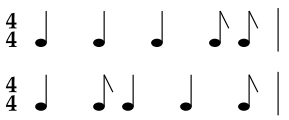
\includegraphics[width=0.4\textwidth]{ch03_symbolic/figures/ioi_comparison.png}
	\end{center}
	\caption[Comparing the identical IOI of two very different rhythms.]{Comparing the identical \acrshort{ioi} of two very different rhythms. Image from \cite{Dixon2004}.}
	\label{fig:ioi_comparison}
\end{figure}


\paragraph{Inter-Onset Interval:} 
Rather than computing the difference between two rhythmic patterns based on the location of the onsets in time, the \acrfull{ioi} summarises a rhythm based on the time elapsed between each onset - or in other words the offset time \citep{Toussaint2013}. For example the clave son would be encapsulated in the string of time elapses as \{3,3,4,2,4\}, using some unit of reference such as 1 = ¼ note. 

Clusters of inter-onset intervals that occur periodically, at a regularly rate that can be quantified per unit time, are referred to by some in the literature as “temporal atoms” or tatum \citep{Bilmes1993, Sethares2007, Jehan2005}. Essentially we can consider the tatum of a score or recording as the fastest note division in which it is written or performed \citep{Sethares2007}. We shall learn later in Chapter 4 that the notion of tatum is important in extracting the tactus or, in musical information retrieval parlance, beat tracking. The computational task of beat tracking involves determining from a signal where a human is likely to tap their foot\footnote{Or more formally, the period at which the conductor swings their baton} when listening to music with a clearly discernable rhythm. 

While \acrshort{ioi}s are unedeniably one of the most important contributors to the impression of accent and pulse perception in music \citep{Parncutt1994}, they are not the most useful feature for comparing rhythms (which is what we are trying to achieve). Firstly as \cite{Dixon2004} correctly point out, two rhythms can have the same distribution of inter-onset intervals, but depending on the length of the notes themselves, the perception of their similarity can turn out to be very dissimilar indeed. In \figref{fig:ioi_comparison} the two rhythms have identical inter-onset intervals but the rhythm above is more typical of a Cha Cha rhythm while the rhythm below is clearly more syncopated and betrays more stylistically that of Rumba.


\paragraph{Chronotonic Distance:} 
Addressing the aforementioned shortcomings intrinsic to \acrshort{ioi}-based comparisons, \cite{gustafson1987new} expands the \acrshort{ioi} representation to a two-dimensional structure that also encapsulates interval time by the integrated area of the rectangle. This elegant depiction allows for clear visual comprehension of rhythmic patterns\footnote{Actually originally intended for scrutiny of rhythm within phonetic study} as we can see in \figref{fig:chronotnic} with the familiar Son. 

\begin{figure}
	\begin{center}
		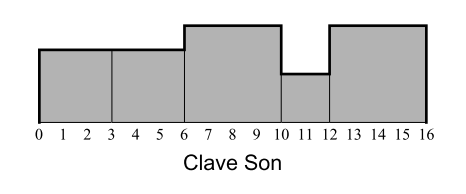
\includegraphics[width=0.65\textwidth]{ch03_symbolic/figures/chronotonic.png}
	\end{center}
	\caption[Chronotic distance of Clave Son]{Chronotic distance of Clave Son. Image from \cite{Toussaint2004}.}
	\label{fig:chronotnic}
\end{figure}

\citep{Toussaint2004} explains how to compare two patterns summarised by their chronotonic distances by treating them as probability distributions and using standard statistical distance measures. While he reports that the chronotonic distance edges past the swap distance based on the criteria of simplicity, goodness of fit, clustering, and ``ancestral'' rhythm generation (rhythms that serve as the seed for many many others), \cite{Guastavino2008} provide experimental evidence that the directed-swap correlates more highly with classically trained musicians’ perceptual impression of dissimilarity when comparing rhythms.

\section{A Genetic Algorithm based on Similarity}

The previous section introduced symbolic representation schemas for rhythm, and symbolic rhythm descriptors, with a particular focus on similarity measures between two rhythms. In this section we will explore how this systematic knowledge can be encapsulated in generative systems. We will begin with a glimpse into some existing relevant work, firstly looking at generative systems that deal with Toussaint style measures of similarity, followed by systems that use genetic algorithms to generate rhythm. Subsequently, we introduce our own proposed work that seeks to specifically merge perceptual measures of rhythmic similarity with genetic or evolutionary algorithms in a system we call GenDrum. We discuss the evaluation of the system and our conclusions that motivates our progression from the symbolic domain to direct content-based analysis and recombination of audio.

\subsection{Generative Rhythmic Systems}

\subsubsection{Generative Rhythmic Systems using Similarity Measures}

Publications dealing with generative applications of symbolic rhythmic similarity exist in the span of literature, but are not so widespread. The Hamming distance, with its easy comprehensible and computable qualities has naturally served a number of systems. \cite{Paiement2007} describe a paper centred around utilising the Hamming distance for generative modelling and prediction of simple rhythms trained in jazz and pop idioms. \cite{Vogl2017} present a tablet application that uses the Hamming distance combined with a restricted Boltzmann machine - a type of artificial perceptron neural network - trained on many drum styles from the Native Instruments Maschine\footnote{\url{https://www.native-instruments.com/en/products/maschine/}} collection. A modified extension has also been extended to database interpolation from that same collection in an earlier  publication \citep{Vogl2016}. Other distance metrics have been exploited less so, and we have found no instances of the directed-swap distance being used in generative tasks.

\subsubsection{Generative Rhythmic Systems using Genetic Algorithms}

Generative systems addressing rhythm with the means of \acrshort{ga} are more abundant. \cite{Eigenfeldt2006a} describes his Kinetic Engine as a software component that generates rhythms in general, not specific to drum sounds. His approach to fitness evaluation is perhaps a controversial one, but not uncommon in musical applications. As in Al Biles’ GenJam system, the role of fitness is simply eliminated. Thus the only real elements of genetic algorithms conserved are crossover and mutation. One may rightfully suspect that such a simplification renders the algorithm commensurate with a randomised search. Consequently a common solution used in such scenarios is to seed the initial population with a known dataset of good input. Another approach could be to embed some rule-based logic that restricts what type of candidates can be generated legally in the seeding process, as we carried out in \citep{Nuanain2014}.

\cite{Bernardes2010} approaches genetic drum pattern generation from the point of view of style emulation. Like Eigenfeldt, they do not incorporate a fitness function, but choose to perform prior analysis on user-supplied or preset MIDI files in a particular style. This process gathers a probability distribution of weighted possible onset times in a 16-step pattern. The population is then seeded with candidates that have patterns generated according to this distribution. 

A short paper by \cite{Horowitz2004a} suggests a multi-dimensional objective fitness function based on the combination of functional evaluations of syncopation, density, downbeat, beat repetition, etc.. Unfortunately the publication is rather scant on actual details regarding the implementation and evaluation of such a method. 

\cite{Kaliakatsos-Papakostas2013} also use the notion of a a target pattern in their evoDrummer software, and define their fitness function by determining what they refer to as divergence in terms of “mean relative distance” to a base rhythm. The distance is computed based on a set of 40 features extracted from patterns, including descriptions of density, syncopation and loudness intensity. Indeed this is perhaps the most related work to our proposed system. 

\begin{figure}
	\begin{center}
		\includegraphics[width=\figSizeHundred]{ch03_symbolic/figures/simpleGA.png}
	\end{center}
	\caption[SimpleGA Pure Data help patch]{SimpleGA Pure Data help patch}
	\label{fig:simplega}
\end{figure}

\subsection{Developing a Genetic Algorithm that can Generate Rhythm}

We set out to design a rhythmically motivated genetic algorithm that was capable of self-evaluation based on the similarity of the patterns it outputs compared to a user-provided seed target pattern. One can envisage this concept being extended to a system that can perform self-evaluation against a previously analysed dataset of patterns that conform to some notion of \textit{style}. 

This section introduces the tools we created in our research: SimpleGA, the genetic algorithm itself that can target the two well known music programming environments \acrshort{pd} and Max, and subsequently encapsulated in the real-time Max for Live instrument GenDrum. Max for Live is an extension of the Max programming environment inhabited in the popular \acrshort{daw} Ableton Live \citep{Manzo2015}. Ableton Live\footnote{\url{https://www.ableton.com/}}, in turn, is one of the most popular \acrshort{daw}s in the dance music community due to its non-linearity and grid-focussed arrangement of loops. 

We continue with a detailed discussion of the implementation of the distance measures and representational issues. Finally there is a description of the design of the experiment for evaluating the research.

\subsubsection{Software Implementation}

SimpleGA is a basic, general purpose genetic algorithm external object we developed for the Pure Data \citep{Puckette1997} and Max/MSP environments in C++ using the cross-platform Flext framework \citep{Grill} . It can handle binary, numerical and alphanumerical strings. A target string is supplied to the object and fitness is determined by measuring its distance to the generated strings using the Hamming or directed-swap distance as was introduced in \secref{sec:distance_measures}. Bang\footnote{The ``bang'' is a fundamental message in \acrshort{pd} and Max that basically means ``do your thing!'' \citep{winkler2001composing}} messages to the leftmost ``hot'' inlet causes the genetic algorithm to undergo a generational stage of evolution, then to output its fittest individual from the pool. \figref{fig:simplega} shows the help patch for the object with this functionality explained visually.

Next we created the GenDrum instrument, a Max for Live device that uses the SimpleGA genetic algorithm to create polyphonic drum patterns of synthesised kick, snare, hi-hat and crash/clap type sounds that emulate the style of a pre-conceived (by input from the user) pattern (\figref{fig:gendrum}). These four sounds are mapped onto a single 16-step row to create a 4x16 drum pattern matrix as is evident in the figure. The operation of the instrument is intended to be as simple as possible. The user inputs a desired pattern into the pattern matrix and assigns this as the target pattern. New target patterns can then be generated by clicking on ``Get New Pattern''. This assigns the best candidate in the current population to the grid and reports its fitness in the number box. In the yellow number box a target fitness can be issued to the genetic algorithm and clicking ``Accelerate!'' will increase the speed of the algorithm until it reaches this target. Patterns that increasingly approach perfect fitness now emerge from the algorithm, repeating and contrasting with the target pattern through repeated stages of \acrshort{ga} evolution.

The instrument also attempts to provide some visual feedback on the evolutionary process using a type of force-directed graph. The fittest individual from each population is represented as a node with its fitness determining the size and distance in relation to the target individual.

\begin{figure}
	\begin{center}
		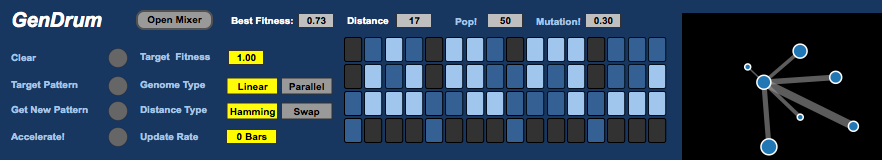
\includegraphics[width=\figSizeHundred]{ch03_symbolic/figures/gendrum.png}
	\end{center}
	\caption[GenDrum main user interface]{GenDrum main user interface}
	\label{fig:gendrum}
\end{figure} 

\subsubsection*{Algorithm Details}

\textit{Linear vs. Parallel Operation}

As the previous section explains, the instrument is intended as a fully functional drum machine, and hence is polyphonic with the possibility of multiple sounds concurring in time. As seen in the literature, similarity studies are predominantly focused with examining monophonic patterns such as the single sound clave son\footnote{The clave son is a two bar measure of either a 3-2 or 2-3 pattern that is integral in many forms of latin dances \citep{Sethares2007}.}. How we deal with the polyphonic implications in our research is outlined here.

Our first naive implementation of the genetic algorithm converts the 4x16 drum pattern matrix into a single “linear'” 64-digit binary string. Evidently this is a simplistic ``brute force'' approach that does not explicitly take into account any musical or perceptual aspect of the application. Specifically it does not embed any knowledge about the constituent sounds and the separation between them in the genome string. Essentially, we’re treating it as a single sound 64-step pattern, with crossover and mutation happening at the halfway point between the first 16 bits of the kick and snare pattern and the second 16 bits of the cymbals/crashes. 

Another approach is to force some kind of logical separation between the different polyphonic timbres in the pattern. By assigning a separate instance of the genetic algorithm to each timbre an overall mean fitness can be derived from the individual outputs. This we implemented and labelled as ``parallel'' mode. Since the genome pattern length is now split from one single 64-bit string to four concurrent 8-bit strings, the time it takes for the genetic algorithms to reach the target fitness is considerably reduced. Some tweaking of the parameters is required to reduce this convergence time and maintain a healthy level of diversity. Setting the population size parameter to 30 and increasing the mutation rate parameter to between 20\% to 40\% has been found to work well in our experience. \figref{fig:genetic} shows the flowchart and design of the GenDrum instrument and it's encapsulation of the SimpleGA \acrshort{ga} in the aforementioned linear and parallel configurations. Next we turn our attention to the distance measures used to derive the fitness function of these genome patterns.

\begin{figure}
	\begin{center}
		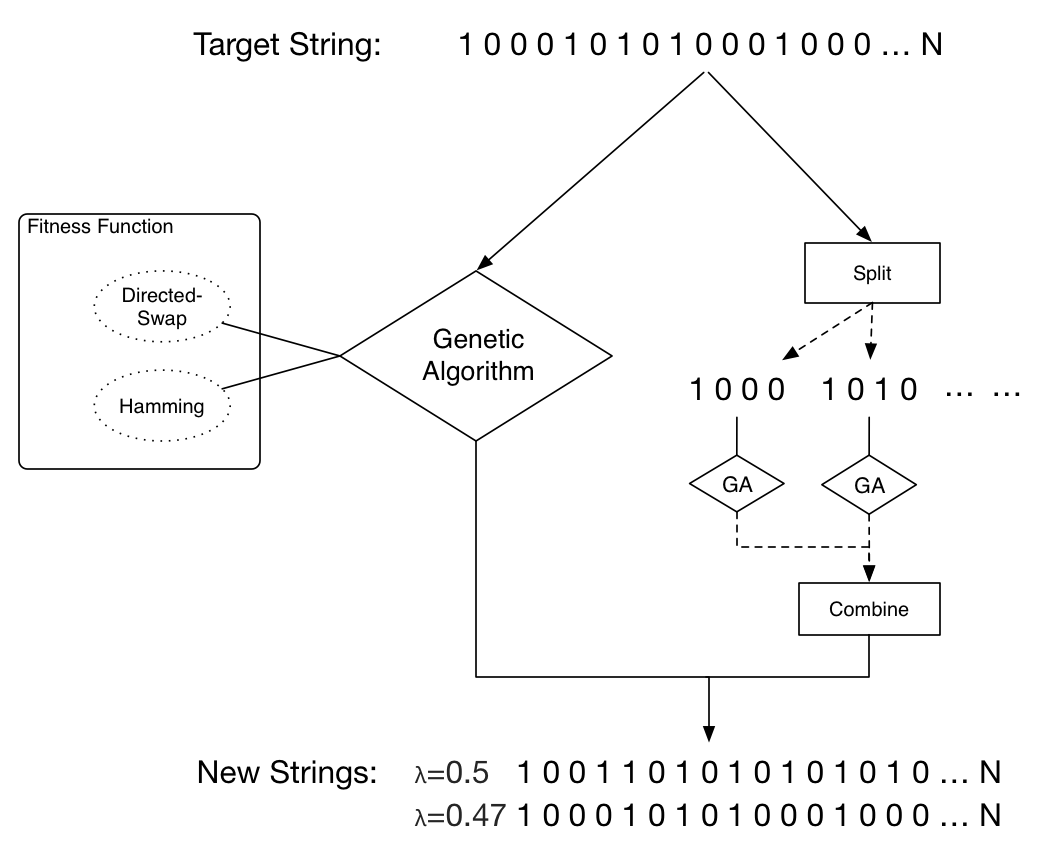
\includegraphics[width=0.8\textwidth]{ch03_symbolic/figures/ga_algorithm.png}
	\end{center}
	\caption[Genetic algorithm flowchart for GenDrum]{Genetic algorithm flowchart for GenDrum. The target string can either be fed to one single \acrshort{ga} (left) or split by timbre, processed by 4 parallel \acrshort{ga}s then recombined (right).}
	\label{fig:genetic}
\end{figure}

\textit{Hamming Distance}

In the review of the state of the art, we referenced how Post and Toussaint have surveyed the effectiveness of the edit distance in determining rhythmic similarity between two binary patterns \citep{Post2011}. Recall that the edit distance allows for insertion, deletion and substitution of symbols within the string. A simplification can be made if operations are restricted to substitutions only, and string lengths are equal (as is always the case in our representations) in which case it becomes the Hamming distance. 

To derive a fitness function using the Hamming distance (\eqnref{eq:fitness_hamming}, using the $\oplus$ exclusive OR operator to determine where the two binary strings are not equal), the number of positions where the two strings $a$ and $b$ match are counted and then divided by the total string length (64 for the linear string and 8 for each string in the parallel implementation). 

\begin{equation}
\label{eq:fitness_hamming}
	f=\frac{1}{N}\sum_{i=1}^{N}a_i \oplus b_i
\end{equation}

\textit{Directed-Swap Distance}

\label{sec:directed_swap}

The Hamming distance takes into account the correct positional scores between two patterns, but it does not give any indicator as to how different a pattern is in terms of the horizontal displacement. Intuitively one would think this horizontal displacement would reflect the important phenomenon of rhythmic syncopation. For example there may exist two different patterns with equal distance, but one pattern has more onsets aligned closer to the original pattern or exhibit a similar distribution of the strong and weak beats in the bar. For these reasons, we decided to test also the directed-swap distance metric as described by \cite{Diaz-Banez2004} in the study of flamenco rhythms, with the hopes that it better captures the spatial comparison between the our generated patterns and the target.

\begin{figure}
	\begin{center}
		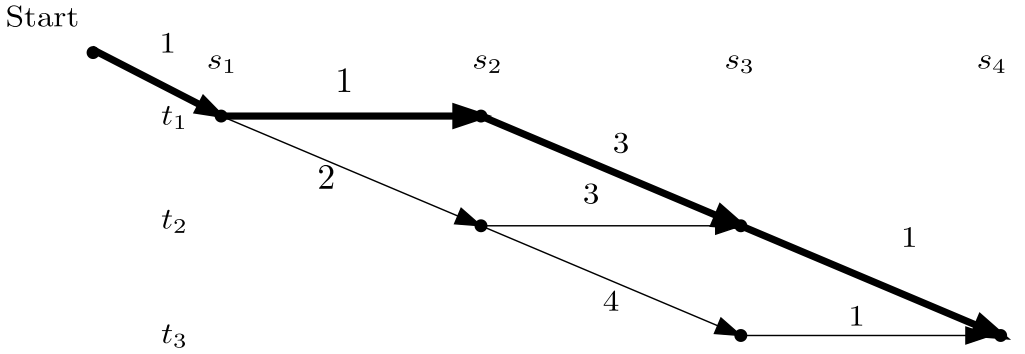
\includegraphics[width=0.75\textwidth]{ch03_symbolic/figures/shortest_path.png}
	\end{center}
	\caption[Solving the directed-swap distance graph for two strings]{Solving the directed-swap distance for strings $A=\{0,2,7,12\}$ and $B=\{1,4,11\}$. Image and example taken from \cite{Colannino2005}}.
	\label{fig:dijkstra}
\end{figure}

Since no implementation existed for the algorithm proposed by \cite{Colannino2005}, we implemented it ourselves, using the Dijkstra implementation in the Boost C++ graph library \citep{Siek2002} to compute the final distance\footnote{\url{https://github.com/carthach/SimpleGA/blob/master/SwapDistance.cpp}}. The derivation and proofs are described at length in their article \citep{Colannino2005} but the basic steps are as follows:

\begin{enumerate}
  \item Convert the two binary rhythms under scrutiny to two sets of indices respectively. For example the pattern $A = \{0, 0, 0, 1, 0, 1, 0, 0\}$ would reduce to the index vector $A = \{3, 5\}$.
  \item Construct a weighted directed acyclic graph from two index vectors $A$ and $B$ by firstly creating the set of vertices $v_{i,j}$ where $1 \leq i \leq |A|$ and $1 \leq j \leq (i+|B|-|A|)$.
  \item For each $v_{i,j}$ add an edge to $v_{i, j+1}$ with weight $|b_{i}-a_{j+1}|$, and an edge to $v_{i+1, j+1}$ with weight $|b_{i+1}-a_{j+1}|$, if $v_{i, j+1}$ and $v{i+1, j+1}$ exist.
  \item Create a start note and add an edge from that node to $v_{1,1}$ with weight $|s_{1}-t{1}|$.
  \item The directed-swap distance is given by the cost shortest path through the graph, solvable with Dijkstra's algorithm (\figref{fig:dijkstra}).
\end{enumerate}

\subsubsection{Operation and Performance}

One way to measure the performance of a genetic algorithm is to plot the fitness values it outputs over a succession of generations. In \figref{fig:genetic} we can see the best fitness and average fitness for all possible configurations of the genetic algorithm over 100 generations. Notice that the linear string representation causes convergence on the target within 40 generations. Notice also that the parallel representation converges prematurely in areas of local maxima, particularly using the swap distance. This can be alleviated through some encouragement of diversity by tweaking the population size and mutation rate.

\begin{figure}
	\begin{center}
		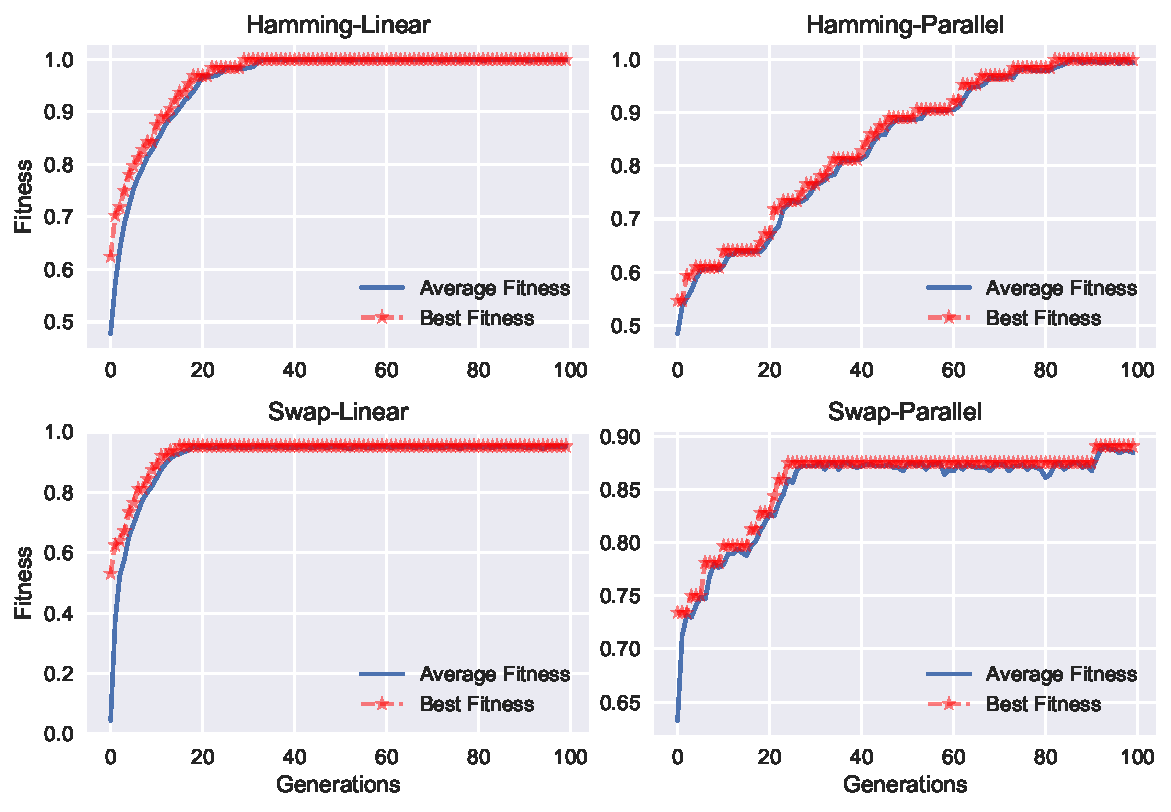
\includegraphics[width=\figSizeHundred]{ch03_symbolic/figures/best_average_fitness.pdf}
	\end{center}
	\caption[Fitness plots for the various configurations of the genetic algorithm]{Fitness plots for the various configurations of the genetic algorithm}
	\label{fig:genetic}
\end{figure}

\subsection{Listener Evaluation \& Discussion}

When evaluating this research and its resulting tools, our goals were to investigate:

\begin{itemize}
	\item The overall correlation of distance with perceived experience.
	\item Comparing the impact of the Hamming distance versus the directed-swap distance on the perceived experience of similarity
	\item Comparing the impact of the linear versus parallel string representation.
	\item The more informal, subjective issue of the musical ``interestingness'' of the rhythmic patterns created.
\end{itemize}


We decided to conduct a simple listening survey to get listener feedback regarding on these aspects. The survey was web-based and unsupervised\footnote{See Appendix \ref{app:listening_survey} for more information}; participants were sent a link with instructions on how to complete it. 

The listening portion of the survey was divided into two parts. The first part examined similarity ratings by presenting the user with the target pattern and the algorithmically generated patterns. Participants were then asked to rate the perceived similarity on a five-point Likert ranging from “Highly Dissimilar” to “Highly Similar”.

The second part then examined the “interestingness” of generated patterns. To enable the participant to ascertain this, the  patterns were arranged in a soundfile as TPx2, GPx2, TPx2, GPx2 (TP=Target Pattern, GP=Generated Pattern) i.e. a two-bar loop of the target pattern is followed by a two-bar loop of a generated pattern and the whole sequence is repeated. This choice of configuration was quite arbitrary, but it was reasoned that in order to get a sense of the interplay between the target pattern and the generated pattern it was necessary to repeat the sequence at least once.

Once again a five-point Likert scale graded the ratings, this time with labels ranging from ``highly disinteresting'' to ``highly interesting''. Regarding the subjective interpretation of ``interestingness'', we instructed the participants to consider how the target pattern and generated pattern ``flows'' from one to another, and how the generated pattern ``develops'' on the target pattern in terms of introducing stimulating variation.

\begin{figure}
	\begin{center}
		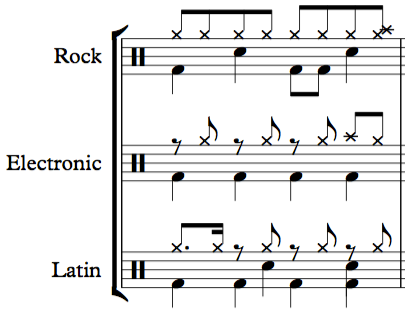
\includegraphics[width=0.6\textwidth]{ch03_symbolic/figures/patterns.png}
	\end{center}
	\caption[Rock, electronic and Son-based patterns used in symbolic listening survey]{Rock, electronic and Son-based patterns used in symbolic listening survey.}
	\label{fig:symbolic_patterns}
\end{figure}

Three target patterns were used for the purposes of the test: a standard straight 8 rock pattern, a four-on-the-floor electronic pattern and a son-based latin pattern (\figref{fig:symbolic_patterns}). \tabref{tab:variable_summary} summarises all the variables under consideration for the evaluation. This resulted in a total of 72 \acrfull{wav} files with 3 fitness levels (inversely corresponding to the distance scores).

{\renewcommand{\arraystretch}{1.5}
\begin{table} 
	\begin{centering}
		\begin{tabular}{c c c c c}
\tabletop
Question & Measure & String & Pattern & Fitness\\	
\tablemid
Similarity & Hamming  & Linear & Rock & Low\\
Interesting & Swap & Parallel & Latin & Med\\
& & & Elec & High\\
\tablebot
		\end{tabular}
		\caption[Listener survey variable summary]{Listener survey variable summary.}
		\label{tab:variable_summary}
	\par \end{centering}
\end{table}

Twenty-two participants took part in the survey, mostly drawn from music students and researchers. All of the participants confirmed that they played an instrument, 7 of whom specified a percussive instrument. Eighteen out of the 22 participants reported the ability to read music. It took approximately 15 minutes to complete.

\subsection{Results}

Before carrying out the statistical analysis the responses were summarised by computing the mode\footnote{Median or mode are generally considered more appropriate measures of central tendency when handling ordinal data such as Likert, and we use Spearman's Rho when performing correlation analysis for similar reason \citep{Boone2012, Lantz2013}.} of the Likert scores for each stimulus. Two “interestingness” stimuli out of the total 72 (36 for similarity, 36 for interestingness) were removed due to high divergence of opinion (50\% or more of the responses deviated by 2 or more Likert scale values from the mode).  

\figref{fig:like1} shows the overall fitness (normalised from its original range of [0-100] to the Likert range [1, 5]) against the mean and standard deviation of the Likert scores by each stimulus. The dip in the middle can be attributed to the different ranges of distance and corresponding fitness produced by the two string measures; the Hamming measure outputs values in a much higher and narrower range. This is more evident looking at the divided plots in \figref{fig:like2} , which plots fitness against Likert scores for each combination of string measure and representation type. 

\begin{figure}
\centering
\begin{subfigure}[b]{0.75\textwidth}
   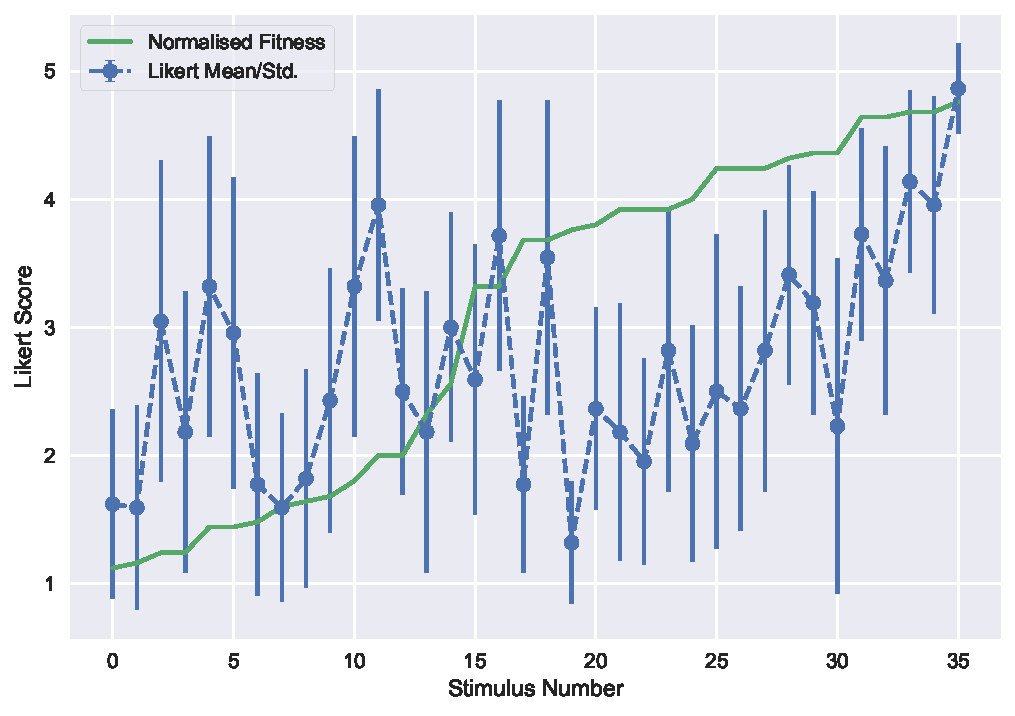
\includegraphics[width=1\linewidth]{ch03_symbolic/figures/total_likert.pdf}
   \caption{}
   \label{fig:like1} 
\end{subfigure}

\begin{subfigure}[b]{0.75\textwidth}
   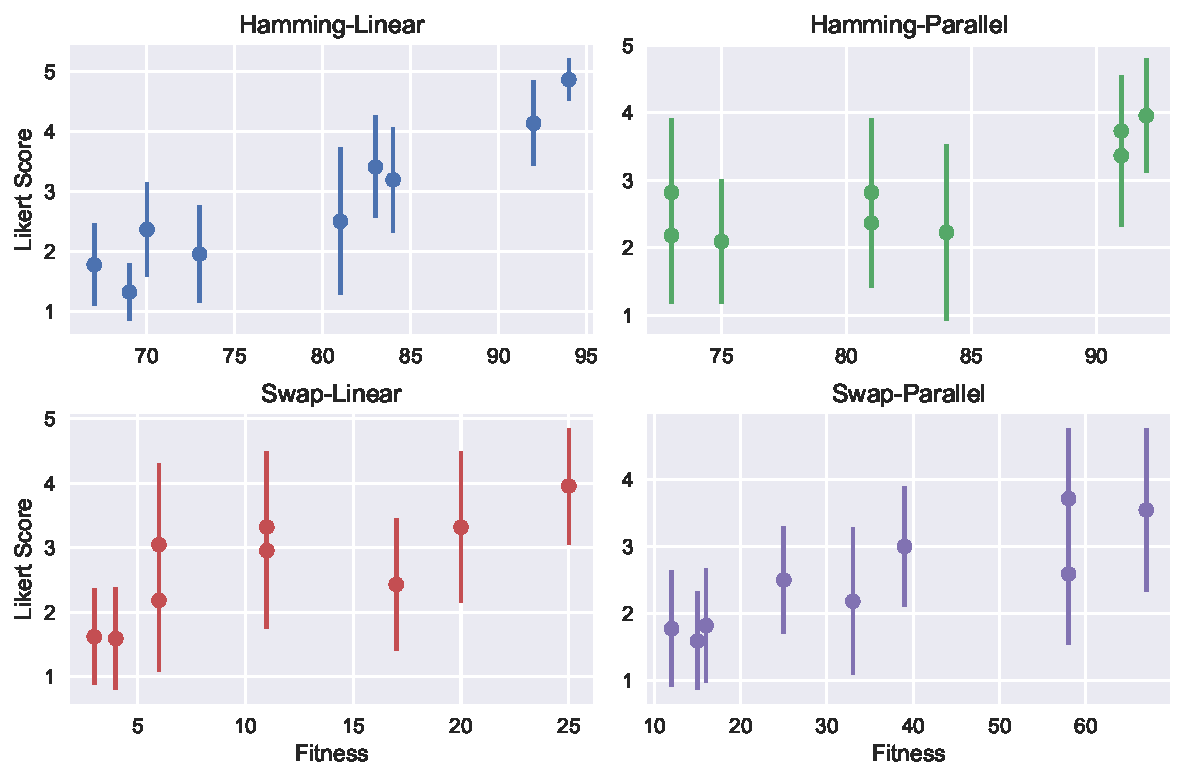
\includegraphics[width=1\linewidth]{ch03_symbolic/figures/separate_likerts.pdf}
   \caption{}
   \label{fig:like2}
\end{subfigure}

\caption[Mean and standard deviation of fitness versus Likert Scores]{Mean and standard deviation of fitness versus Likert scores for (a) each stimulus (b) measure and string type.}
\end{figure}
\subsubsection{Similarity Ratings}

Our first task when looking at the data was to confirm whether inverse pattern distance and the fitness of the genetic algorithm correlates with the perceived similarity as determined by the participants. 

The data appears to suggest that this hypothesis is confirmed. \tabref{tab:overall_similarity_correlation} presents the Spearman ranked correlation matrix of fitness, distance and the mode scores received for each stimulus. There is a clear, strong negative correlation coefficient (\(\rho\) = -0.71, p < 0.05) between the distance measure and the perceived similarity to the target.  This correlation is not as clear with the fitness function, which can be attributed to the fact that fitness as a function of distance is evaluated differently for the two distance measures.

{\renewcommand{\arraystretch}{1.5}
\begin{table} 
	\begin{centering}
		\begin{tabular}{c | c c c}
\tabletop
& Distance & Fitness & Score\\	
\tablemid
Distance & 1.0000 & -0.4145 & -0.7134\\
Fitness & -0.4145 & 1.0000 & 0.4353\\
Score & -0.7134 & 0.4353 & 1.0000\\
\tablebot
		\end{tabular}
		\caption[Overall similarity correlation matrix]{Overall similarity correlation matrix}
		\label{tab:overall_similarity_correlation}
	\par \end{centering}
\end{table}

\figref{fig:hamming_versus_swap} shows the separated distance and fitness correlations against the mode scores for the Hamming and directed-swap distance measures. The fitness correlation values are 0.784 and 0.625 respectively and the distance correlation values are -0.784 and -0.716 respectively (p < 0.05). It can be seen that the Hamming distance has slightly better correlation.

\begin{figure}
	\begin{center}
		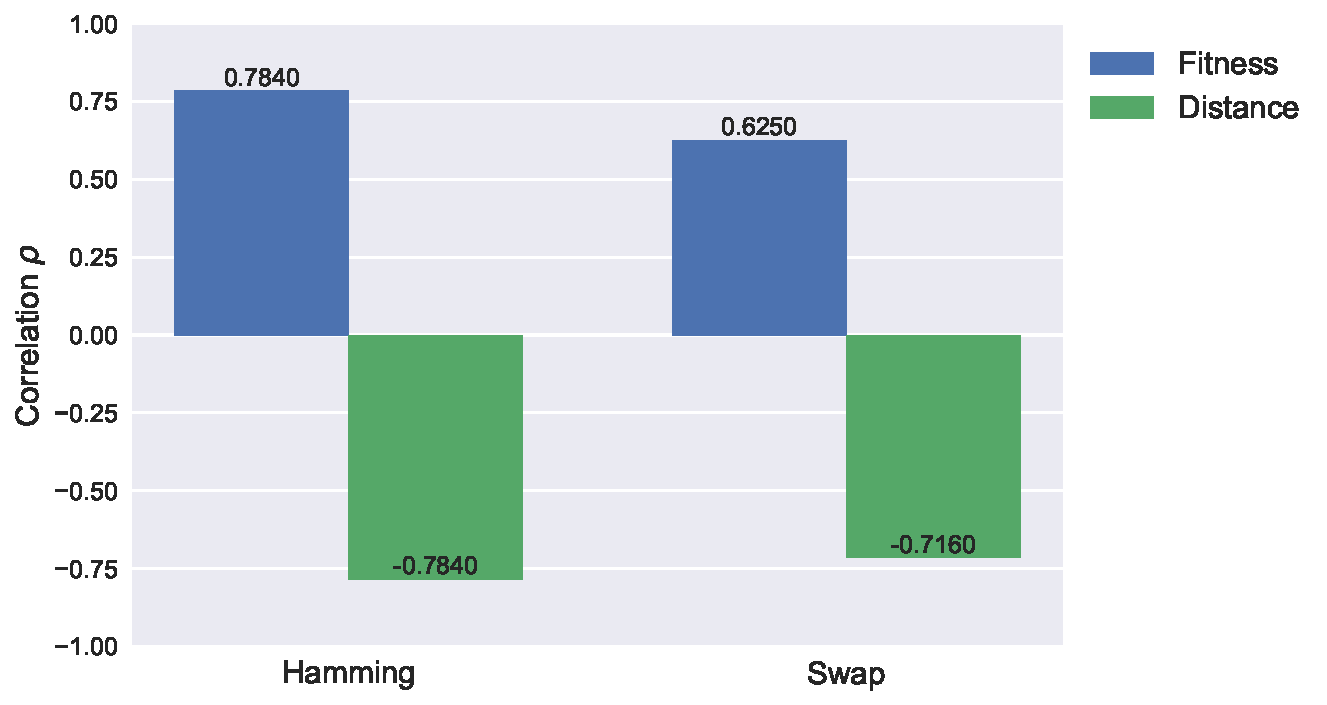
\includegraphics[width=0.75\textwidth]{ch03_symbolic/figures/measure_bar.pdf}
	\end{center}
	\caption[Fitness and distance for Hamming and swap distance metrics]{Fitness and distance for Hamming and swap distance metrics}
	\label{fig:hamming_versus_swap}
\end{figure}

\figref{fig:linear_versus_parallel} shows the separated distance and fitness correlations against the scores when we discriminate between linear and parallel pattern strings. The fitness correlation values are 0.525 and 0.480 respectively, and the distance correlation values are -0.852 and -0.576 respectively (p < 0.05). The linear representation scheme appears to correlate better with human judgement.

Post hoc analysis using a t-test and a Kruskal-Wallis non-parameteric \acrshort{anova} H-test compared the two different conditions - linear vs. parallel and hamming vs. directed-swap - and discovered a significant difference for the ratings of the distance measure (p < 0.05), but not in the case of the string representation type. Out of interest, we also examined the participants' musical experience in reading notation or playing a percussive instrument, but they had no significant effect on the ratings (p > 0.05) in both instances.

We can draw some tentative conclusions based on this data. Firstly, the strong correlation between the overall distance and similarity ratings suggest that, even for polyphonic string representations of drum patterns, distances such as the Hamming and directed-swap are useful measures of perceived similarity. Secondly, splitting and recombining the bit strings by timbre, as carried out in the parallel operation, does not seem to offer improvement over the simplistic, long bit string representation. Finally, the more complex directed-swap algorithm, with its ability to capture the ``horizontal'' displacement between two drum patterns, does not appear to reflect an increase in similarity scores in our survey, confirming Toussaint's finding but also extending it to the case of polyphonic patterns.

\begin{figure}
	\begin{center}
		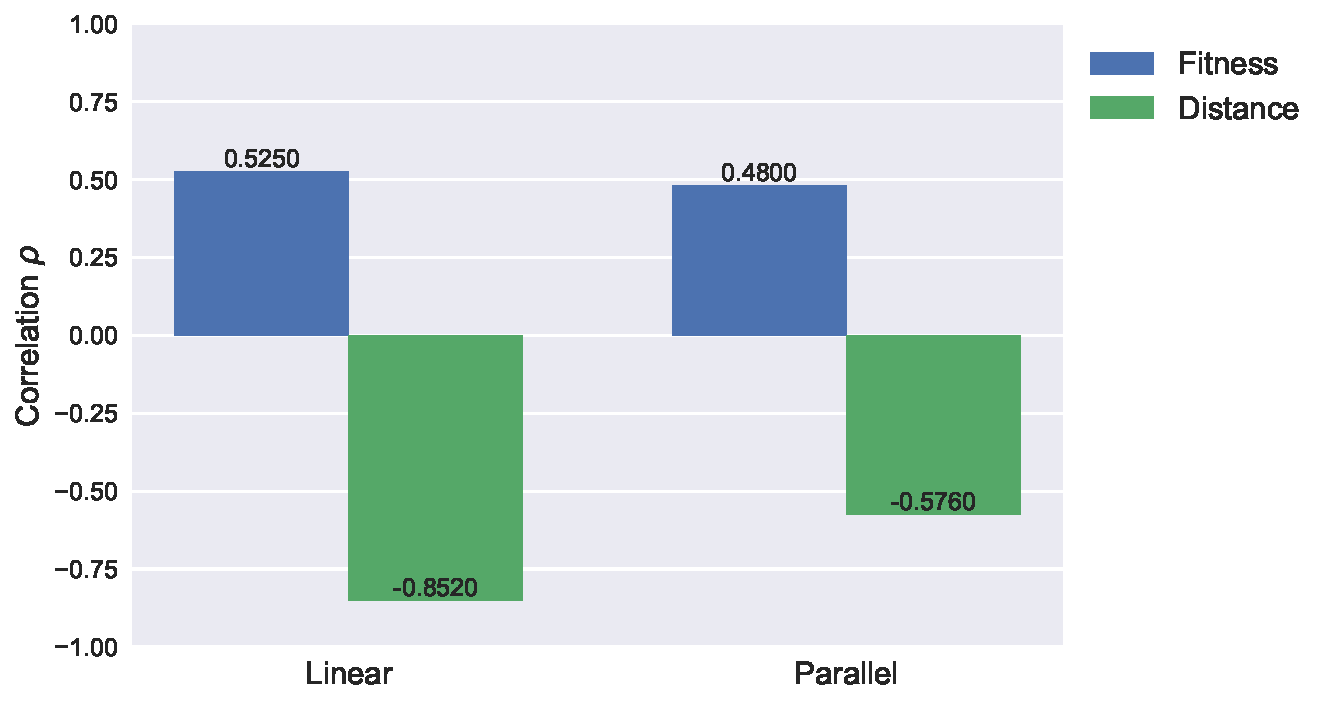
\includegraphics[width=0.75\textwidth]{ch03_symbolic/figures/reps_bar.pdf}
	\end{center}
	\caption[Fitness and distance for linear and parallel string computation]{Fitness and distance for linear and parallel string computation}
	\label{fig:linear_versus_parallel}
\end{figure}


\subsubsection{Subjective “Interestingness” Evaluation}

\tabref{tab:interestingness} presents the correlation matrix corresponding to the results of the users' impression regarding the "interestingness" of the patterns when heard in a sequence with the target. Curiously, the distance and fitness correlation coefficients are both positive, despite the fact that distance is inversely proportional to the fitness of the genetic algorithm but the p-values are so high (0.211 and 0.1887 respectively) that this data is not reliable. It is impossible to draw some meaningful or significant conclusions based on the disparity and inconsistency across subjects.

Disregarding the difficulty in appraising musically subjective output, the reason for this problematic data is largely attributable to the way in which we considered the notion of ``interestingness'' and how the question was formulated. Asking the participants to rate two essentially diametrically opposing qualities - i.e. variation (related to dissimilarity) and repetition (related to similarity) was a flawed approach that caused confusion. This became immediately apparent from some of the user feedback at the end of each survey session. For example:

\blockquote{\textit{“I noticed that I somehow prefer rhythms that are a natural
evolution of the previous pattern, instead of being totally different. But if the similarity with the previous pattern is too high, the result is still uninteresting to me, because the resulting pattern is too predictable and loses every appeal.”}}

To complete the survey then, users often reverted to their own rules to determine their ratings, as evident from these comments:

\blockquote{\textit{“Interestingness” was hard for me to evaluate. In the end I rated with a `good' interesting `bad' interesting system: if it's weird but i like it, it's in the first case, if not, in the second case.''}}

\blockquote{\textit{“.. There are some times on experiment 2 that the new rhythm might not be interesting for a complete section but that might be useful as a bridge or as a temporal loop marking the end of a section."}}

Another participant made the point that the pattern sequence may have forced some `expectation' regarding the concept of “interestingness”:

\blockquote{\textit{“... I have also the feeling that having the pattern repeated (ie AB twice), and therefore, having to come back to A again after having been in B, conditions very much the results.”}}

{\renewcommand{\arraystretch}{1.5}
\begin{table} 
	\begin{centering}
		\begin{tabular}{c | c c c}
\tabletop
& Distance & Fitness & Score\\	
\tablemid
Distance & 1.0000 & -0.5419 & 0.2201 \\
Fitness & -0.5419 & 1.0000 & 0.2310 \\
Score & 0.2201 & 0.2310 & 1.0000 \\
\tablebot
		\end{tabular}
		\caption[`Interestingness' correlation matrix]{`Interestingness' correlation matrix}
		\label{tab:interestingness}
	\par \end{centering}
\end{table}

Despite the apparent issues with our method of evaluation, the data and informal feedback does suggest that the genetic algorithm creates “interesting” musical output. Nineteen stimuli out of the 34 analysed registered a mode score value higher than 4 as seen by the 56\% green positive region in \figref{fig:interesting_distribution} (there were two responses for “Strongly Disagree”, but these were the two that were disregarded due to high divergence of opinion). The task ahead is to review the evaluation strategy in order to quantify and explain this aspect in a more coherent and predictable manner, decoupling the interdependency of the questioning between similarity and interdependence.

\subsection{Improving the System - Adding More Features}

\begin{figure}
	\begin{center}
		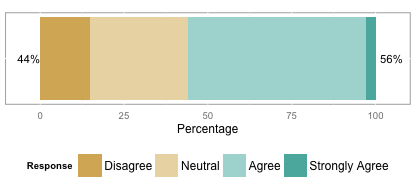
\includegraphics[width=0.75\textwidth]{ch03_symbolic/figures/interestingness.png}
	\end{center}
	\caption[Distribution of responses for `interestingness' in symbolic evaluation]{Distribution of responses for `interestingness'.}
	\label{fig:interesting_distribution}
\end{figure}

The evaluation shows that our implemented methods do behave predictably in returning increasingly similar patterns to a target as the mean fitness of the genetic algorithm converges on its maximum. It also shows, despite deficiencies in the mode of questioning, that listeners do perceive these patterns favourably, given the sounds used and some localised awareness of style.

However we still felt that similarity methods alone were not capturing all of the subtleties inherent in symbolic rhythm patterns, features that other systems might include that prove more fruitful in analysis and generation. Another iteration of development on the genetic algorithm included three additional improvements that are described here.

\subsubsection{Timbre Weighting}

\label{sec:timbre_weighting}

Other than allowing the separation of the pattern into its constituent timbres for discrete generation in the parallel mode, our generative system makes no additional effort to extrapolate and delineate the obvious hierarchical and emergent roles the separate timbres induce in the sensation of drum patterns. 

Our brains process rhythm streams with different timbres and spectral profiles differently, and awareness and study of this fact goes some of the way to explaining why across different styles and cultures dispersion of timbres exhibit similar proportions across different frequency bands. To be precise we often see liberal placement of high-frequency, short attack timbres like hi-hats across all beats, while the kick drum usually enforces the downbeat\footnote{Let's forget about reggae for now!} and start of bar and finally the mid-range snare drums fills in the backbeat\footnote{Jazz and rock music attribute far greater importance to the backbeat though, which, much to the irritation of musicians, is not obvious to all concertgoers who insist on clapping on the `one and three' (\url{http://www.ethanhein.com/wp/2013/the-backbeat-a-literature-review/}). A very entertaining video shows a live concert where pianist Harry Connick Jr. uses rhythmic displacement to insert a bar of 5/4 in a 4/4 piece of music. This intentionally shifts the clapping audience from `one and three' to the `two and four' backbeat, much to the relief and gratitude of the drummer! (\url{https://www.youtube.com/watch?v=--qv9SI6vws)}}. As \cite{Merchant2015} observes in the general scope of pop music 

\blockcquote[]{Merchant2015}{``\textit{...the vast majority of drum patterns in popular music have bass drum hits on the downbeat (e.g. beats 1 and 3 of a 4/4 pattern) and snare hits on the upbeats (beats 2 and 4). While not inviolable, this statistical generalization leads listeners familiar with these genres to have strong expectations about how to assign musical events to a particular metrical position, thus using learned top-down cognitive processes to reduce the inherent ambiguity of the musical surface.}''}

Other researchers also point to the salience of the kick and snare drums in the inference of downbeats and upbeats in rhythm perception and, consequently, its computational analysis \citep{Zils2002, Panteli2014a, Gomez-Marin2017}. Leaving aside \textit{why} exactly this is the case \footnote{\cite{Hove2014} proposes that ``its our superior time perception for lower musical pitch''.}, it is clear that not all drum timbres are created equal, and generative systems such as ours should incorporate some cognisance of that important fact.

To remedy this, a weighting scheme was used to assign different degrees of importance to the separate timbre streams when operating in parallel mode. The exact formulation weights are not important, just that they are weighted sufficiently to bias the fitness function as desired, so for example we weigh the 4 streams successively from bottom (kick) to top (perc or cymbal) with  the set $W = \{2, 1, 0.5, 0.25\}$. These weights are also parametric to account for different timbres assigned to the different streams.

\subsubsection{Syncopation}

\blockcquote[]{Toussaint2013}{``\textit{Syncopation is the spice of rhythm}''}

Just as musical ideas blossom through the balance between repetition and variation of a motif or loop, rhythms are made infinitely interesting by resolving the tension arising from anticipation and reinforcement of the beat and the deliberate disruption of that expectation. The \textit{Harvard Dictionary of Music} defines syncopation simply as:

\blockcquote[]{Apel1969}{``\textit{Syncopation: a momentary contradiction of the prevailing meter or pulse}''}

\cite{Gomez2005} expand on this definition:

\blockquote{\textit{``Moreover, syncopation can be materialized either as a momentary change of the primary character of the meter or as a contradiction between strong and weak beats against other parts of the musical texture whose metrical context is fixed''}}

Up until now, our algorithm has only been considering the similarity of generated rhythms in relation to the target, and has no facility to gauge the level of syncopation present in the target or the generated rhythms. It would be a useful parameter of the \acrshort{ga} to allow the user to increase bias for selecting candidates based on relative syncopation of strong and weak beats in a particular track, and this was the next feature that was implemented.

\cite{Eigenfeldt2013} incorporate a rudimental quantifier for level of syncopation into their hybrid rhythm algorithm by simply counting the number of onsets that do not fall on the expected strong beats in the metre (4/4).

To expand our system to include knowledge of syncopation, we turned once again to perceptual literature to see if there were any established analytic methods that prove more grounded in observation rather than blindly devising our own. \cite{Gomez2005} sum up 4 such measures including:

  \begin{figure}
	\begin{center}
		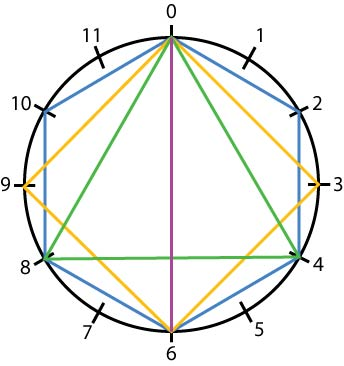
\includegraphics[width=0.3\textwidth]{ch03_symbolic/figures/offBeatness.jpg}
	\end{center}
	\caption[Toussaint's Off-Beatness measure]{Toussaint's Off-Beatness measure. Image from McGill.}
	\label{fig:offbeatness}
	\end{figure}
	
\begin{itemize}
  \item The Rhythmic Oddity Property \citep{arom2004african} is not really a measure, it is simply a boolean value indicating whether there exists two onsets in a pattern that divide the set equally or not.
  \item Toussaint's \textit{Off-Beatness} \citep{Toussaint2004African} finds those geometric shapes that divides an $N$ length rhythm necklace evenly (\figref{fig:offbeatness}). These are the on-beats. The number of onsets that lie outside of these geometric entities give the degree of off-beatness.
  \item Keith's Measure \citep{keith1991polychords} defines syncopation in terms of three events, \textit{hesitation} (a note starts on a beat but ends off a beat), \textit{anticipation} (a note starts off a beat but ends on a beat) and \textit{syncopation} as a combination of of hesitation and anticipation within a rhythm. Weights are assigned to these three event categories (like our own timbre weightings used in \secref{sec:timbre_weighting}, these are subjective by the author) and the weighted sum of instances of these constitute the measure of syncopation in the measure.
\end{itemize}}

\cite{Gomez2005} criticises Keith's measure in its arbitrary assignment of weights but, more crucially, its restriction to binary metres (explained in depth the article). They offer a new measure to address these limitations and coalesce some elements inherent in Toussaint's off-beatness. The key tenet of the \acrfull{wnbd} is that ``notes are supposed to end where the next note starts''. Onsets that land off strong beats are given the smaller weighting and weighting increases to a maximum as notes cross over strong beats - which they posit gives the strongest sensation of syncopation. 

\blockcquote[]{Gomez2007}{\textit{``the closer a note is to a strong beat, the more syncopated it sounds; and second, the syncopation effect is stronger when a note crosses over only one strong beat of the meter.''}}

While \cite{Song2013} has some reservations of this model and we could find no instances of surveys that evaluated its correlation with human listeners, it does seem a reasonable distillation of syncopation for our purposes, compared to the other formulations.  \acrshort{wnbd} is distance-based model that can be easily integrated into our fitness function with comparative ease.  Based on a reference implementation offered in Synpy \citep{Song2015}, a Python environment for syncopation modelling, we expanded the genetic algorithm to include the \acrshort{wnbd} in its fitness function.

\subsubsection{Density}

The density of a rhythm is an easy feature to comprehend, \cite{Wiggins2012a} defines it as the ``mean number of events per tactus beat''. We simply added another metric for the fitness function to consider, given by the average number of onsets per pattern (\eqnref{eq:density}), where $x_i$ is onset number $i$ and $N$ is the total number of onsets.

\begin{equation}
\label{eq:density}
	d(x)=\frac{\sum_{i=1}^{N}x_i}{N} \quad \text{if}\ x_i=1
\end{equation}

\begin{figure}
	\begin{center}
		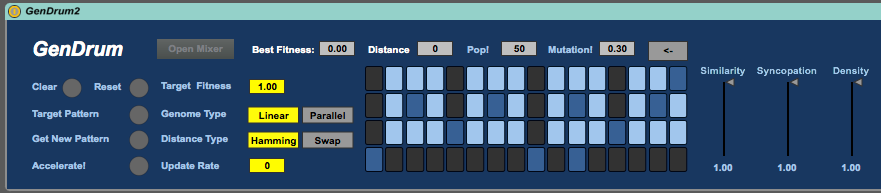
\includegraphics[width=1.0\textwidth]{ch03_symbolic/figures/gendrum2.png}
	\end{center}
	\caption[GenDrum interface with expanded feature parameter control]{GenDrum interface with expanded feature parameter control to the right.}
	\label{fig:gendrum2}
\end{figure}

Having influence over density in a generative drum machine is a desirable control to have and  has actually been shown to be a useful descriptor in modelling rhythmic similarity, specifically in dance music signals \citep{Panteli2014a}. Within the GiantSteps project the Agnostic Density Transformer \citep{Jorda2016} is a generative drumming system that is focussed on density control of individual drum sounds based on corpus analysis, and has since been expanded into a mobile app by Reactable Systems\footnote{\url{https://reactable.com/snap/}}.

The weighted linear combination of these three features coupled with the new parallel timbre weighting scheme comprise the new fitness function for the genetic algorithm. Since these additional features represent a considerable departure from the general string analytics offered by the SimpleGA object, we decided to encapsulate it in a separate, specialised object called RhythmGA. \figref{fig:gendrum2} shows the revised interface for GenDrum that uses the new \acrshort{ga}, along with the new similarity, syncopation and density  sliders that adjust the relevant parametric weights.

\subsection{Conclusions and Closing Remarks}

In this chapter we presented a way of generating drum patterns automatically using genetic algorithms. Rather than relying on the commonly used interactive fitness function, our method was shown to use the notion of a “target pattern”, with fitness derived from the distance of the generated patterns to the target. This was devised to address the way dance music composers derive tracks from a bottom-up approach that begins with a small loop or idea that is iteratively expanded through repetition and variation of its key features.

Following a review of various approaches to establishing the distance between rhythms as present in the literature, we demonstrated the implementation and incorporation of two such measures - the Hamming distance and the directed-swap distance - into a genetic algorithm instrument for polyphonic drum pattern creation. We believe this work, and the accompanying articles, constitute the first integration of perceptual symbolic similarity research in rhythmic pattern generation with genetic algorithms.

To evaluate the research carried out, we conducted a listening survey to determine participants' reaction to the generated patterns in terms of the similarity and “interestingness” related to the target pattern. It was shown that the distance ,and thus fitness, correlates strongly with user perception in terms of similarity. Crucially we showed that the Hamming distance alone is a worthwhile quantifier of rhythmic similarity even in the case of polyphonic patterns. Our approach to gauging users' response to the concept of  “interestingness”, however, needs review and presents a complex challenge for future work. 

Based on the feedback ascertained during the evaluation, a second iteration of the genetic algorithm along with the accompanying instrument was developed that assimilated an expanded feature set as well as enhanced parametric control for the user. By adjusting these parameters, relative weightings of rhythmic attributes such as similarity, syncopation and densities can bias the fitness function as appropriate. While our own informal appraisal of these additions was favourable, a more rigorous evaluation and listening survey was not conducted. This was due to a shift of focus away from symbolic algorithm composition towards approaches involving content-based, \acrshort{mir}-driven synthesis of real audio.

The reasons for this change of tack were multifold. Firstly, while genetic algorithms coupled with an appropriately formulated fitness function demonstrably provide a legitimate mechanism for generating rhythms for dance music, methods proposed by our colleagues that invoke specialised metrics \citep{Marin2015} or knowledge trained on large corpora representing style \citep{Jorda2016} are perhaps more suited. This has been confirmed in a collaborative evaluation conducted by ourselves along with others in the GiantSteps consortium \citep{Vogl2016}. Our \acrshort{ga} did not fare better in various listening tests against neural networks and a database-driven method both trained on human derived patterns from the Maschine software and hardware environment (and understandably so, as the two methods indisputably embed more knowledge). However it did return more ``interesting'' results and was rated higher in its facility for creating more unique fill patterns. 

%Article dealing with Listener Surveys from MuMe
%
%Agres, K., Forth, J., \& Wiggins, G. A. (2016). Evaluation of musical creativity and musical metacreation systems. Computers in Entertainment, 14(3), 1–33. https://doi.org/10.1145/2967506

But most of all, based on an overall critique of the myriad approaches to generating rhythms using symbolic conventions and similarity analysis (including our own experiences building systems that utilise them), we sensed that there are some subtleties inherent in real recordings and performances of rhythms that are not encapsulated via these means. Namely we could identify:

\begin{itemize}
\item The notion of verticality or interdependence between concurrent elements at discrete points in time that are not completely captured by concepts such as metrical hierarchy and weighting.
\item Stress and accents that affect the dynamics of onsets in a pattern, not captured by the pervasion of binary representations that exists in literature and associated realised systems. This perhaps can be addressed by analysing and estimating rhythms in terms of real or floating point numerical forms.
\item Related to stress and accents there are other difficult phenomena of human factors in music that include groove and swing. These are notoriously difficult facets to define and quantify by musicologists, and even harder to estimate and recreate using computational means. The need to replicate human qualities of time within conventional music production systems is clear however. Most \acrshort{daw}s at least include some ability to adjust metrical positioning of note information according to some percentage factor ostensibly tantamount to groove.
\item The timbral qualities - or the sounds and processing used to derive the patterns - we contend have a profound impact on the perceptual response and aesthetic impression of the loop. Simply assembling rhythms according to perceptual similarity measures using arbitrary sounds (all too frequently coarse \acrshort{midi} approximations) does not always produce the desired results, at least in generative attempts at dance music.
\end{itemize}

All these factors were carefully considered and it became more apparent that perhaps the symbolic domain was not sufficient for our goals. The focus of the thesis turns to investigating whether these methods can be refined, adapted and extended to systems that generate rhythms using signals and thus connecting time with timbre.